\documentclass[letterpaper,12pt,oneside,final]{book}
%%
%%  Gabarit de mémoire de maîtrise ou thèse de doctorat.
%%  Template for dissertations and theses @ Polytechnique Montreal.

%%  Normalement, il n'est pas nécessaire de modifier ce document
%%  sauf pour établir le langage (français ou anglais) et pour changer les noms des 
%%  fichiers à inclure.
%%  Usually, this document needs to be modified only to set up the language (French or English) 
%%  and to change the names of the files to include.
%%
%%  Version: 2018-07-31
%%
%%  Accepte les caractères accentués dans le document (UTF-8).


\makeatletter
\def\bstctlcite{\@ifnextchar[{\@bstctlcite}{\@bstctlcite[@auxout]}}
\def\@bstctlcite[#1]#2{\@bsphack
 \@for\@citeb:=#2\do{%
   \edef\@citeb{\expandafter\@firstofone\@citeb}%
   \if@filesw\immediate\write\csname #1\endcsname{\string\citation{\@citeb}}\fi}%
 \@esphack}
\makeatother

% LA COMMANDE SUIVANTE ÉTABLIT LE LANGAGE DE LA THÈSE : ÉCRIRE french POUR UNE THÈSE EN FRANÇAIS
% THE NEXT COMMAND DETERMINES THE LANGUAGE OF THE THESIS: WRITE english FOR A THESIS IN ENGLISH
\newcommand\Langue{french}            

\usepackage{ifthen}
\usepackage[utf8]{inputenc}
%%
%% Support pour l'anglais et le français (français par défaut).
%\usepackage[cyr]{aeguill}
\usepackage{lmodern}      % Police de caractères plus complète et généralement indistinguable visuellement de la police standard de LaTeX (Computer Modern).
\usepackage[T1]{fontenc}  % Bon encodage des caractères pour qu'Acrobat Reader reconnaisse les accents et les ligatures telles que ffi.

% le langage par défaut est le dernier de la liste, c'est-à-dire français
\ifthenelse{\equal{\Langue}{english}}{
	\usepackage[french,english]{babel}
}{
	\usepackage[english,french]{babel} 
}

%%
%% Charge le module d'affichage graphique.
\usepackage{graphicx}
\usepackage{epstopdf}  % Permet d'utiliser des .eps avec pdfLaTeX.
%%
%% Recherche des images dans les répertoires.
\graphicspath{{./images/}{./dia/}{./gnuplot/}}
%%
%% Un float peut apparaître seulement après sa définition, jamais avant.
\usepackage{flafter,placeins}
%%
%% Utilisation de natbib pour les citations et la bibliographie.
%\usepackage{natbib}
%%
%% Autres packages.
\usepackage{amsmath,color,soulutf8,longtable,colortbl,setspace,xspace,url,pdflscape,cite}
%%
%% Support des acronymes.
\usepackage[nolist]{acronym}
\onehalfspacing                % Interligne 1.5.
%%
%% Définition d'un style de page avec seulement le numéro de page à
%% droite. On s'assure aussi que le style de page par défaut soit
%% d'afficher le numéro de page en haut à droite.
\usepackage{fancyhdr}
\fancypagestyle{pagenumber}{\fancyhf{}\fancyhead[R]{\thepage}}
\renewcommand\headrulewidth{0pt}
\makeatletter
\let\ps@plain=\ps@pagenumber
\makeatother
%%
%% Module qui permet la création des bookmarks dans un fichier PDF.
%\usepackage[dvipdfm]{hyperref}
\usepackage{hyperref}
\usepackage{caption}  % Hyperlien vers la figure plutôt que son titre.
\makeatletter
\providecommand*{\toclevel@compteur}{0}
\makeatother
%%
%% Définitions spécifiques au format de rédaction de Poly.
%% Here we define the Poly formatting.
\RequirePackage[\Langue]{MemoireThese}
%%
%% Définitions spécifiques à l'étudiant.
%% -----------------------------------
%% ---> À MODIFIER PAR L'ETUDIANT / TO BE MODIFIED BY THE STUDENT <---
%% -----------------------------------
%%
%% Commandes qui affichent le titre du document, le nom de l'auteur, etc.
\newcommand\monTitre{Conception, fabrication et test d'une roue Cyr haute performance}
\newcommand\monPrenom{Charlotte}
\newcommand\monNom{Dubost}
\newcommand\monDepartement{génie mécanique}  % Department
\newcommand\maDiscipline{Génie mécanique}
\newcommand\monDiplome{M}        % (M)aîtrise ou (D)octorat / (M)aster or Ph(D)
\newcommand\anneeDepot{2020}    % Year
\newcommand\moisDepot{Juillet}       % Month
\newcommand\monSexe{F}           % "M" ou "F" = Gender
\newcommand\PageGarde{N}         % "O" ou "N" = Yes or No
\newcommand\AnnexesPresentes{O}  % "O" ou "N". Indique si le document comprend des annexes. / If the thesis includes annexes = O or N = No.
\newcommand\mesMotsClef{Cirque,roue,cyr,composites,elasticité}
\usepackage{gensymb}
%%
%%  DEFINITION DU / OF JURY
%%
%%  Pour la définition du jury, les macros suivantes sont definies:
%%  \PresidentJury, \DirecteurRecherche, \CoDirecteurRecherche, \MembreJury, \MembreExterneJury
%%
%%  Toutes les macros prennent 3 paramètres: Sexe (M/F), Nom, Prénom
%%  All the macros have 3 parameters: Sex (M/F), Last name, First name
\newcommand\monJury{\PresidentJury{F}{Nom}{Prenom}\\
\DirecteurRecherche{M}{Gosselin}{Frédérick}\\
\CoDirecteurRecherche{F}{Ross}{Annie}\\
\CoDirecteurRecherche{M}{Therriault}{Daniel}\\
\MembreJury{M}{Nom}{Prénom}\\
\MembreExterneJury{M}{Nom}{Prénom}}


\ifthenelse{\equal{\monDiplome}{M}}{
\newcommand\monSujet{Mémoire de maîtrise}
\newcommand\monDipl{Maîtrise ès sciences appliquées}
}{
\newcommand\monSujet{Thèse de doctorat}
\newcommand\monDipl{Philosophi\ae{} Doctor}
}
%%
%% Informations qui sont stockées dans un fichier PDF.
\hypersetup{
  pdftitle={\monTitre},
  pdfsubject={\monSujet},
  pdfauthor={\monPrenom{} \monNom},
  pdfkeywords={\mesMotsClef},
  bookmarksnumbered,
  pdfstartview={FitV},
  hidelinks,
  linktoc=all
}
%%
%% Il y a un document par chapitre du mémoire.
%%
\begin{document}
\bstctlcite{IEEEexample:BSTcontrol}

%%
%% Page de titre du mémoire.
\frontmatter
% Compte optionellement la page de garde dans la pagination.
\ifthenelse{\equal{\PageGarde}{O}}{\addtocounter{page}{1}}{}
\thispagestyle{empty}%
\begin{center}%
\vspace*{\stretch{0.1}}
\textbf{POLYTECHNIQUE MONTRÉAL}\\
affiliée à l'Université de Montréal\\
\vspace*{\stretch{1}}
\textbf{\monTitre}\\
\vspace*{\stretch{1}}
\textbf{\MakeUppercase{\monPrenom~\monNom}}\\
Département de~{\monDepartement}\\
\vspace*{\stretch{1}}
\ifthenelse{\equal{\monDiplome}{M}}{Mémoire présenté}{Thèse présentée} en vue de l'obtention du diplôme de~\emph{\monDipl}\\
\maDiscipline\\
\vskip 0.4in
\moisDepot~\anneeDepot
\end{center}%
\vspace*{\stretch{1}}
\copyright~\monPrenom~\monNom, \anneeDepot.
%%
%% Identification des membres du jury.
%%
\newpage\thispagestyle{empty}%
\begin{center}%

\vspace*{\stretch{0.1}}
\textbf{POLYTECHNIQUE MONTRÉAL}\\
affiliée à l'Université de Montréal\\
\vspace*{\stretch{2}}
Ce\ifthenelse{\equal{\monDiplome}{M}}{~mémoire intitulé}{tte thèse intitulée} :\\
\vspace*{\stretch{1}}
\textbf{\monTitre}\\
\vspace*{\stretch{1}}
présenté\ifthenelse{\equal{\monDiplome}{M}}{}{e}
par~\textbf{\mbox{\monPrenom~\MakeUppercase{\monNom}}}\\
en vue de l'obtention du diplôme de~\emph{\mbox{\monDipl}}\\
a été dûment accepté\ifthenelse{\equal{\monDiplome}{M}}{}{e} par le jury d'examen constitué de :\end{center}
\vspace*{\stretch{2}}
\monJury
%%
\pagestyle{pagenumber}%
%% Dédicace
%%
%% La dédicace est un hommage que l'auteur souhaite
%% rendre à une ou plusieurs personnes de son choix.
%%
\ifthenelse{\equal{\Langue}{english}}{
	\chapter*{DEDICATION}\thispagestyle{headings}
	\addcontentsline{toc}{compteur}{DEDICATION}
}{
	\chapter*{DÉDICACE}\thispagestyle{headings}
	\addcontentsline{toc}{compteur}{DÉDICACE}
}

\begin{flushright}
  \itshape
  A ceux qui mettent leurs connaissances et compétences au service de l'art, et à ceux qui cherchent un moyen de le faire. 
  \ldots
\end{flushright}
          % Dédicace du document.
% Remerciements / Acknowledgements
%
%  Grâce aux remerciements, l'auteur attire l'attention du lecteur
% sur l'aide que certaines personnes lui ont apportée, sur leurs
% conseils ou sur toute autre forme de contribution lors de la
% réalisation de son mémoire. Le cas échéant, c'est dans cette section
% que le candidat doit témoigner sa reconnaissance à son directeur de
% recherche, aux organismes dispensateurs de subventions ou aux
% entreprises qui lui ont accordé des bourses ou des fonds de
% recherche.
\ifthenelse{\equal{\Langue}{english}}{
	\chapter*{ACKNOWLEDGEMENTS}\thispagestyle{headings}
	\addcontentsline{toc}{compteur}{ACKNOWLEDGEMENTS}
}{
	\chapter*{REMERCIEMENTS}\thispagestyle{headings}
	\addcontentsline{toc}{compteur}{REMERCIEMENTS}
}
%
Merci à mes directeurs de recherche, Frédérick Gosselin, Annie Ross et Daniel Therriault pour l'énergie et le temps qu'ils ont accordé à l'accompagnement de ce projet ainsi que pour leur vivacité d'esprit et l'excellence de leurs expertises dont j'ai eu la chance de bénéficier. \\\\
Merci à Marion Cossin pour son soutien, ses précieux conseils et son appui au sein de l'Ecole Nationale de Cirque de Montréal dès le début du projet.\\\\
Merci à toute l'équipe de l'Ecole Nationale de Cirque pour sa collaboration.
     % Remerciements.
% Résumé du mémoire.
%
\chapter*{RÉSUMÉ}\thispagestyle{headings}
\addcontentsline{toc}{compteur}{RÉSUMÉ}

La roue Cyr est un agrès de cirque composé d’une roue métallique à la géométrie torique dont le diamètre avoisine la hauteur de l’utilisateur et dont le poids varie de 10kg à 20kg. L’utilisateur se place au centre de la roue, s’y agrippe et effectue des figures acrobatiques tout en tournant. Ceci fait du poids et de la rigidité des facteurs déterminants pour la performance de l’utilisateur. Depuis son invention cet agrès a été revisité plusieurs fois par des artistes et des fabricants d’équipement de cirque. En particulier, depuis que l’utilisation de matériaux avancés (comme la fibre de carbone) est devenue populaire pour les équipements sportifs, et qu’elle commence à être adopté par certains fabricants pour les mats et les portiques, la communauté circassienne manifeste de l'intérêt pour les possibilités nouvelles qu’une roue Cyr plus légère et plus flexible pourrait apporter. La géométrie torique d’une roue Cyr rend sa fabrication plus compliquée et le prototypage plus couteux, parmi les projets de roue Cyr en matériaux composites, aucun n’a été mené à bien, pour cause manque de moyens où d’absence de modélisation théorique. En outre, développer une modélisation dynamique de la roue Cyr (dont le mouvement est similaire à celui du disque d’Euler) nécessite de se plonger dans une étude approfondie.
Le but de ce projet est donc de déterminer de quelle manière l’utilisation de matériaux composites pour la fabrication d’une roue Cyr enrichira la discipline, aussi bien en termes de possibilités acrobatiques que de jeu de scène, ainsi que d’identifier des propriétés mécaniques et géométries optimisées correspondant aux mouvements et aux efforts exercés sur une roue Cyr.



Le déroulement du projet est basé sur la méthodologie suivante:
\begin{itemize}
\item Étude théorique : Développement d’un modèle mathématique des mouvements caractéristiques de la roue Cyr et du stockage d’énergie, des sauts et rebonds. Une fois que le modèle est établi, caractérisation des paramètres géométriques et mécaniques déterminants ainsi que de leur influence. Développement d’une analyse adimensionnelle et d’une loi d’échelle.
\item Étude numérique : développement d’un modèle numérique des mouvements de la roue Cyr en utilisant Python.
\item Preuve de concept : Une fois que les propriétés optimales ont été déterminées imprimer en 3D une petite portion de la roue, de même rayon de courbure, avec le matériau correspondant. Une fois que cette portion est testée et validée, imprimer un modèle réduit et le tester adéquatement à l’aide de la loi d’échelle déterminée à l’étude théorique.
\item Prototypage à l’échelle 1
\item Test du prototype : En partenariat avec l’École Nationale de Cirque de Montréal.
\end{itemize}

Le projet contribue à l’avancement des connaissances dans différents domaines et pour des communautés diversifiées : en plus de compléter certaines recherches concernant le disque d’Euler, ou plus globalement les disques et les tores en rotation ou les anneaux élastiques, ce qui fait l’originalité et l’importance du projet réside dans l’apport de nouvelles connaissances à la communauté circassienne : les fabricants d’équipement de cirque auront une réponse concernant l’intérêt de la fabrication de roue Cyr en matériaux composites, ainsi qu’un exemple de procédé de fabrication et, (surtout !) pour les artistes et metteurs en scène la discipline se verra enrichie par de nouvelles possibilités et de nouvelles opportunités de création.

      % Résumé du sujet en français.
% Abstract
%
% Résumé de la recherche écrit en anglais sans être
% une traduction mot à mot du résumé écrit en français.

\chapter*{ABSTRACT}\thispagestyle{headings}
\addcontentsline{toc}{compteur}{ABSTRACT}
%

The Cyr Wheel is a circus apparatus consisting of a 2 meters diameter (size may vary with the height of the user) ring made of steel or aluminum, with a weight varying between 10kg and 20kg. The user stands inside the wheel and performs acrobatic tricks while spinning. This utilization makes the weight, rigidity and geometry determinant influence parameters for the way the user will perform on the wheel. Since its invention in 1996 it has been revisited several times by circus artists and manufacturers, and especially with the utilization of advanced materials for sport equipment spreading to circus structures (such as poles and gantries), the circus community shows interest for the possibilities that a lighter, more flexible Cyr wheel could bring (like jumping and bouncing with the wheel, for instance). The fact that a Cyr wheel is made of curved elements leads to a significant increase in terms of fabrication costs, and none of the Cyr wheel projects involving new composite materials has been completed to this day, mostly because of a lack of means, and the fact that it is too expensive to get to the right prototype by the ‘trial and error’ method. On the other hand, developing a theoretical model of the dynamics of Cyr wheel is a complex task which requires an in-depth study since its motion can be linked to the Euler’s disk model. 
For now, advances on this question consist in trials of prototypes manufactured with no prior theoretical studies which resulted in a lack of optimization and unsuitable material choices leading to failure when tested.\\ 

To this day there aren’t any scientific publications specific to the Cyr wheel dynamics or the use of composite materials for circus structures. Nevertheless, Euler’s disk and spinning coins have been widely studied by the scientific community due to the chaotic aspect of their motion in its terminal stage as well as the influence of friction and air viscosity on its behavior. The mathematical model developed to study this problem provide a basis that will be adapted the dimension, shape and use of the Cyr wheel. The ability to jump with the Cyr wheel being a determinant aspect of the study, the model developed by Yang and Kim about energy storage in elastic rings will also be used as a basis an adapted to the scale and problematics specific to a Cyr wheel.\\

Carrying out the study of a composite Cyr wheel from its design to the test and validation of a prototype requires to combine at the same time practical knowledge of the apparatus, theoretical knowledge about composite materials, 3D printing processes and dynamics of Euler’s disk-like motions, as well as mastery of numerical modelling and large scale composite 3D printing equipment. These conditions are hard to reunite at once, which explains why, contrary to other circus apparatuses, the question of the use of composite materials for Cyr wheel manufacturing has not been solved yet and why no scientific publication has been released on this subject. Answering this problematic represents a significant evolution of the discipline of Cyr wheel and of the manufacturing of this apparatus. On top of that, it will allow to bring quantitative answers to multiple questions that have only be tackled intuitively until then.\\
The general objective of this study is to estimate the mechanical properties and geometry that will allow to optimize and diversify the use of a Cyr wheel, choose a corresponding material to 3D print the Cyr wheel in, print a real size prototype and experiment on the new acrobatic possibilities of this new apparatus.

The guidelines of the project are the following research questions:
\begin{itemize}
\item What would be the optimal material properties (Young modulus, density) and geometry that would expand the acrobatic possibilities of a Cyr wheel ? 
\item	How would this circus discipline evolve with a corresponding Cyr wheel made out of a high-performance optimized material ? 
\end{itemize}
\\
\\
\\

The project is based on the following hypothesis:\\
Developing a Cyr wheel with a rigidity and a weight different from the existing ones will significantly contribute to the evolution of the discipline.\\
This hypothesis will be refuted if the new acrobatic tricks that we suppose this new type of Cyr wheel will allow are too demanding (physically or in terms of skills) and can’t be achieved by a professional Cyr wheel performer, even with some practice time.\\

Justification of the originality: Considering the dynamics of a spinning Cyr wheel with a performer, adding elastic properties and a lighter weight sounds promising and has been tried several times, but never achieved.\\
Success criteria: a successful contribution would consist in advances in the theoretical knowledge of Cyr wheel, by quantitatively answering problematics raised by the circus community, evolution of the discipline by expanding the acrobatic possibilities of this apparatus and providing answers concerning the interest of the introduction of composite materials for Cyr wheels to manufacturers.\\

The project will be carried out with the following methodology:

\begin{enumerate}
\item Theoretical study:
develop a mathematical model of Cyr wheel motions and of energy storage, jumping and bouncing. Once the model is established, identify the parameters of significant influence among material properties and geometry parameters (Young modulus, density, moment of inertia, size of diameter…). Study the scalability and develop an dimensionless analysis.

\item Numerical study:
develop a numerical model of Cyr wheel motions, study the dynamic stability and energy storage capability. Quantify the influence of the identified parameters by studying the impact of their variation on the motion.

\item Proof of concept:
once the optimal properties of the material are estimated thanks to the two previous phases, develop a corresponding composite material and 3D print a small part of the wheel with the same radius of curvature than the real-size one. Once it is tested and validated, print a small size prototype and test it applying appropriate strength estimated with the scalability study.

\item Real size prototyping:
3D-print the final prototype: a real size Cyr wheel made out of the optimized high performance composite material previously defined

\item Test of the prototype:
validate that the chosen material is appropriate.
Explore the news acrobatic possibilities provided by the prototype.

\end{enumerate}


The impacts and benefits of the project are the following:
\begin{itemize}
\item Carrying out this study will allow circus equipment manufacturers to further the reflection and conclude on the pros and cons of adding composite Cyr will to their current offer.
\item Developing a numerical model of Cyr wheel motions will allow to quantify the influence of different parameters such as rigidity, density and geometry on the performance of the user. This will bring an answer to problematics left unanswered until now such as the ones put forward by the research department of Montreal National Circus School (ideal user’s weight/ Cyr wheel weight ratio, ideal user’s height, Cyr wheel diameter ratio) 
\item The resulting research article will provide a basis for further investigation about the Cyr wheel, since no publication has been released on this topic to this day.
\item On a broader perspective, this study will be a contribution to advances in the research on sporting equipment involving circular shapes and problematics of lightness and flexibility.

\end{itemize}
          % Résumé du sujet en anglais.

{\setlength{\parskip}{0pt}
%%
%% Table des matières.
\ifthenelse{\equal{\Langue}{english}}{
	\renewcommand\contentsname{TABLE OF CONTENTS}
}{
	\renewcommand\contentsname{TABLE DES MATIÈRES}
}
\tableofcontents
%%
%% Liste des tableaux.
\ifthenelse{\equal{\Langue}{english}}{
	\renewcommand\listtablename{LIST OF TABLES}
}{
	\renewcommand\listtablename{LISTE DES TABLEAUX}
}\listoftables
%%
%% Table des figures.
\ifthenelse{\equal{\Langue}{english}}{
	\renewcommand\listfigurename{LIST OF FIGURES}
}{
	\renewcommand\listfigurename{LISTE DES FIGURES}
}\listoffigures
%%
%% Liste des annexes au besoin.
}

% Liste des sigles et abbréviations / List of acronyms and abbreviations
\ifthenelse{\equal{\Langue}{english}}{
	\newcommand\abbrevname{LIST OF SYMBOLS AND ACRONYMS}
}{
	\newcommand\abbrevname{LISTE DES SIGLES ET ABRÉVIATIONS}
}
\chapter*{\abbrevname}
\addcontentsline{toc}{compteur}{\abbrevname}
\pagestyle{pagenumber}
%
\begin{acronym}
  \acro{ENC}{Ecole Nationale de Cirque}
  \acro{FEDEC}{Fédération Européenne Des Ecoles de Cirque professionnelles}
\end{acronym}
%
\begin{longtable}{lp{5in}}
ENC       & Ecole Nationale de Cirque\\
\end{longtable}

       % Liste des sigles et abréviations.
\ifthenelse{\equal{\AnnexesPresentes}{O}}{\listofappendices}{}
\mainmatter
% Dans l'introduction, on présente le problème étudié et les buts
% poursuivis. L'introduction permet de faire connaître le cadre de la
% recherche et d'en préciser le domaine d'application. Elle fournit
% les précisions nécessaires en ce qui concerne le contexte de
% réalisation de la recherche, l'approche envisagée, l'évolution de
% la réalisation. En fait, l'introduction présente au lecteur ce
% qu'il doit savoir pour comprendre la recherche et en connaître la
% portée.

\Chapter{INTRODUCTION}\label{sec:Introduction}  % 10-12 lignes pour introduire le sujet.
Texte en \emph{italique}, \textsc{petites majuscules}, mot \mbox{insécable}.\\
Texte \ul{souligné}, \hl{surligné}, \textbf{gras}.\\
Texte entre ``guillemets''.\\
Police \texttt{monospace}.\\
Un mot courant en réseautique mobile: n\oe{}ud\footnote{Note de bas de page.}.\\
L'objet RSVP \texttt{SENDER\_TEMPLATE}.\\
%Nom d'un auteur: \citeauthor{RFC_IPv4}.\\
Une architecture 32~bits.\\
\\
Support d'acrobatie, entrainant le corps de l'utilisateur qui s'y accroche dans un mouvement de rotation, mais pouvant aussi bien être manipulée par ce dernier, la roue Cyr se place à mi-chemin entre les disciplines acrobatiques, les disciplines d'équilibrisme et la manipulation d'objet. La réalisation de figures acrobatiques repose sur un équiibre dynamique continuel entre la roue et le corps de l'utilisateur: ce dernier influe sur le mouvement de la roue, tout en modulant le rythme et la force qu'il applique en fonction des caractéristiques de la roue (sa masse, son inertie, sa géométrie). Un changement dans ces caractéristiques rend ainsi nécessaire l'adaptation de l'artiste à une variation du mouvement. La popularité croissante de l'utilisation de matériaux composites pour la fabrication d'équipement de cirque comme les mats ou les portiques éveille l'intérêt de la communauté circassienne sur les possibilités nouvelles qu'une roue Cyr faite d'un tel matériau peut apporter. L'enjeu est double: le procédé de fabrication offrant un éventail de possibilités géométriques inaccessibles avec les métaux ainsi qu'un choix des propriétés mécaniques beaucoup plus large, on y voit une occasion d'optimiser les mouvements déjà existants mais aussi d'inventer de nouvelles figures avec une roue Cyr faite d'un matériau dont les propriétés élastiques permettent, par exemple, de sauter avec la roue.
%%
%%  CONCEPTS DE BASE / BASIC CONCEPTS
%%
\section{Définitions et concepts de base}  % environ 2-3 pages



\subsection{Définitions}
\paragraph{Circassien(ne):} relatif au cirque 
\paragraph{Agrès de cirque:} équipement nécessaire à la pratique d'une discipline circassienne. Exemples: la roue Cyr, le trapèze, le tissu aérien, les cannes d'équilibre, le mat chinois...
\paragraph{Disque d'Euler:} disque ayant un mouvement de rotation similaire à celui d'une pièce qu'on fait tourner sur une surface plane. Lorsque son mouvement entre en phase terminale sa vitesse de rotation augmente de façon impressionnante, ce qui lui a valu de devenir un jouet éducatif, mais aussi de faire l'objet de nombreuses publications scientifiques. Son mouvement est similaire à un des mouvements caractéristiques de la roue Cyr.


\subsection{Historique de la roue Cyr}
La roue Cyr que l'on retrouve dans les spectacles de cirque contemporains doit son  nom à Daniel Cyr, qui fabriqua sa première roue en 1996 \cite{Inertie}. A cette dernière, faite en une seule pièce d'acier recouverte d'un revêtement en PVC afin d'améliorer l'adhérence avec le sol, succéda rapidement  une roue Cyr démontable en plusieurs parties. La première apparition marquante de la roue Cyr sur la scène circassienne eut en 1998 dans un spectacle du Cirque Eloize, dont Daniel Cyr est le co-fondateur. Une médaille d'argent remportée en 2003 par ce dernier au Festival Mondial du Cirque de Demain acheva d'assoir la popularité de ce nouvel agrès dans le secteur du cirque, mais également en tant que sport.\\
Cependant l'idée d'une roue à la géométrie torique dont le diamètre avoisine la taille humaine remonte bien avant la création de Daniel Cyr \cite{Inertiehist,gymmedia,howstuffwork}. En effet, plusieurs agrès d'apparence similaire à celle de la roue Cyr ont fait leur apparition du côté de l'Allemagne dès le début du vingtième siècle. On remarquera en particulier l'Einrefen, inventé en 1930 par Adalbert von Rekowski, qui diffère de la roue Cyr par des poignées intérieures pour les mains et les pieds. \\
Depuis, la roue Cyr continue d'évoluer, comme le montrent les agrès dérivés présentés à la fin du manuel de la FEDEC (Fédération Européenne Des Ecoles de Cirque professionnelles) \cite{Fedec2011}. Les procédés de fabrication se sont eux aussi affinés \cite{corbin}, et les roues Cyr lumieuses programmables ont vu le jour.\\
La fabrication en matériaux composites se présente aujourd'hui comme l'étape suivante dans l'évolution de l'agrès.

\subsection{Les figures de roue Cyr}
Nous présentons ici les figures de roue Cyr constituant la base principale de la discipline. Ces dernières, ainsi que d'autres figures plus approfondies sont détaillées dans le manuel de la FEDEC \cite{Fedec2011}
\subsubsection{La valse (ou pas de base)}
Le corps est positionné de façon symétrique, avec bras et jambes chacun inclinés à 45\degree de la verticale. L'utilisateur initie la rotation d'une poussée du pied puis accompagne le mouvement de la roue en utilisant le tranfert de son poids, tirant et poussant successivement la roue dans le sens de la rotation.\\
Ce mouvement se décline en plusieurs variations en ajoutant par exemple un lacher de pieds, qui avec un arc de cercle de la jambe devient un arabesque, ou encore en l'exécutant à une seule main ou mains croisées, en serrant et croisant les jambes ou en les écartant jusqu'au grand écart latéral. Cette figure s'exécute aussi avec un pied placé sur la roue au niveau de la tête, en grand écart facial. On peut aussi varier en jouant avec la position du corps: corps de profil, dans le plan de la roue, arqué vers l'intérieur, tendu vers l'extérieur...

\subsubsection{Les tours}
Dissociation du mouvement: la roue tourne mais pas le corps. Ce type de figure peut être exécuté en effectuant un demi-tour, un tour complet, ou même un tour en suspension avec l'utilisateur suspendu à la roue par une main.

\subsubsection{Les vrilles}
Dissociation inverse, le corps tourne dans le reférentiel de la roue. De même ce type de figure se décline en diverses sortes de demi vrilles et en vrille complète en suspension.

\subsubsection{Les suspensions}
Comme l'indique le nom, les pieds ne sont pas sur la roue. On peut par exemple exécuter la valse en suspension, sans les pieds, ou simplement prendre de l'élan puis lacher les pieds et adopter une position groupée en tournant sur place, ce qui a pour effet d'augmenter la vitesse de rotation. Il est possible de se suspendre par une ou deux mains, par les coudes, les bras tendus ou fléchis. La suspension est la base de la figure du Superman: corps gainé, jambes tendues vers l'extérieur de la roue.

\subsubsection{Le drapeau}
La roue n'est tenue que par la main et le pied d'un même côté. La rotation est alimentée en poussant et tirant avec la main et le pied restant, tout en tendant puis groupant successivement la main et le pied lachés.

\subsubsection{Les sauts}
La roue tourne sur elle même, l'utilisateur saute et prend appui come il le souhaite, bras tendus, pliés, ou même en position assise sur la roue. Il peut ensuite atterrir sur le sol ou directement sur la roue.

\subsubsection{Le corner ou inclinaison horizontale}
L'utilisateur se décale sur un côté de la roue jambes serrées, prend appui jambes fléchies puis plonge vers le sol, jambes tendues le corps se retrouve en position horizontale pour un demi tour. Cette figure peut se réaliser en lachant un bras, un pied, ou un bras et un pied simultanément.

\subsubsection{Le saut de mains}
L'utilisateur pousse la roue vers le sol avec une main, accompagne le renversement avec son poids, ouvre les doigts quand sa main arrive au niveau du sol puis la tire au dessus de sa tête et la pousse avec ses jambes afin de revenir à l'endroit. Cette figure s'exécute en avant, en arrière, en position de profil, à une jambe.

\subsubsection{La roue}
L'utilisateur exécute une roue classique tout en étant dans la roue au moyen de transferts de poids. Il est possible de réaliser cette figure en enchainant plusieurs roues le long d'une trajectoire circulaire, ou bien d'une ligne droite. Il est possible de la combiner avec d'autres figures et changements de directions et d'enchainer ainsi plusieurs roues dans des sens différents.

\subsubsection{La pièce}
Ce mouvement est semblable à la rotation d'une pièce de monnaie (ou du disque d'Euler) dans la phase terminale du mouvement. L'utilisateur, gainé, ouvre sucessivement les doigts pour ne pas les écraser lorsque ses mains arrivent au niveau du sol, et transfere son poids pour accompagner le mouvement et l'alimenter aussi longtemps qu'il le souhaite. Cette figure peut s'exécuter à différentes hauteurs du sol, plus la pièce est basse, plus la vitesse sera élevée. On peut aussi la réaliser à l'envers, le corps arqué (pièce dorsale).

\clearpage

%%
%lt% anément eELEMENTt chent la roue simuS DE LA PROBLEMATIQUE
%%
\section{Problématique}  % environ 3 pages
La création d'une roue Cyr en matériaux composites, aux propriétés différentes de celles qui roues Cyr métalliques, qui permettra d'enrichir la discipline de nouvelles figures se trouve au carrefour de la science, de la technique acrobatique et de l'art. Ceci nécessite de réunir des expertises issues de ces différents domaines, couplés à des moyens de fabrication adéquats. La problématique peut donc se découper selon les trois étapes caractéristiques du projet.

\subsection{Conception}
Il s'agit de déterminer quels paramètres parmi les propriétés mécaniques du matériau et la géométrie de la roue Cyr influencent de manière notable les mouvements de cette dernière, puis de caractériser cette influence quantitativement. \\ 
A cet effet des modèles théoriques de deux mouvements caractéristiques ont été développés:
\begin{itemize}
    \item Le saut (la possibilité d’intégrer des sauts aux figures de roue Cyr déjà existante étant une des lignes directrices du projet): la roue est compressée par l'exercice d'une force dont l’axe coincide avec le diamètre, puis relâchée. Une part de l’énergie élastique stockée est convertie en saut. 
    \item Le mouvement correspondant à celui d’une pièce de monnaie qui roule sur sa tranche en décrivant des cercles, puis entre en phase terminale avant de tomber à plat sur le sol.
\end{itemize}

En se basant sur chacun des modèles théoriques correspondants, l’objectif est de déterminer séparément les paramètres géométriques et mécaniques qui :
\begin{itemize}
    \item  permettent à l’utilisateur de sauter le plus haut possible avec la roue.
    \item permettent d’optimiser le mouvement similaire à celui de la pièce de monnaie décrit ci-dessus en termes de stabilité dynamique.
    \item conduisent au meilleur compromis entre les deux réponses aux questions précédentes.
\end{itemize}


Parallèlement, il est indispensable d’étudier les contraintes et déformations dans la roue et plus particulièrement celles dues à l’impact avec le sol lors des sauts afin d’identifier des zones de design, qui garantissent que cette dernière ne sera pas endommagée.

\subsection{Fabrication}
Il s’agit de compléter l’étude théorique issue de la phase de conception par une utilisation adaptée de l’impression 3D. En utilisant les technologies existantes et disponibles pour le projet, comment imprimer un tore d’un diamètre avoisinant les deux mètres ? Comment assurer des propriétés conformes à celles déterminées par les modèles théoriques établis au préalable ? 

\subsection{Tests}
Malgré la popularité du sujet au sein de la communauté circassienne et des pratiquants de roue Cyr, la roue en matériaux composites ne figure pas parmi les offres des fabricants d’équipement de cirque. Ces dernières sont en partie influencées par le fait qu’il y ait un flou, une difficulté à estimer concrètement ce qu’apporterait une telle roue Cyr et donc si les individus adeptes de la discipline seraient prêts à acquérir une roue Cyr composite, pour un prix bien supérieur à ceux des roues métalliques. En effet, leur fabrication nécessite un investissement conséquent qui ne peut être fait sans avoir de certitude sur sa rentabilité. Une phase de recherche artistique menée avec le prototype à l’échelle 1 imprimé et fonctionnel et en collaboration avec des artistes de roue Cyr de haut niveau, permettra de lever le voile sur les nouvelles possibilités introduites par une roue Cyr composite, aussi bien en termes d'acrobaties que de jeu de scène, ainsi que sur la réaction de la communauté et des pratiquants, ce qui permettra aux fabricants d'évaluer plus clairement si une véritable demande peut exister.\\
En outre, plusieurs artistes de roue Cyr ont déjà tenté d'approcher ces nouvelles possibilités, avec des roues Cyr fabriquées de manière artisanales dans des matériaux plus légers ou plus flexibles (par exemple une roue Cyr en osier a été fabriquée par des élèves au Centre National des Arts du Cirque (CNAC) en France)
cependant ces projets d'expérimentation n'ont pu être menés à terme, les roues se retrouvant rapidement endommagées et hors service. Ceci s'explique par le manque de moyens et de temps à consacrer à une étude préalable méthodique et approfondie rassemblant des expertises diverses et des moyens de fabrication adéquats, ainsi qu'une maitrise des procédés de fabrication additive. Fournir un prototype fonctionnel et solide permettra à ces artistes de continuer et d'approfondir leur recherche dans la sécurité, au terme de quoi la discipline pourrait prendre un nouveau tournant.\\


% On veut éviter que la figure et le tableau soient placés au-delà de la section courante.
\FloatBarrier


%%
%% OBJECTIFS DE RECHERCHE / RESEARCH OBJECTIVES
%%
\section{Objectifs de recherche}  % 0.5 page
\subsection{Objectif global}
L'objectif global de ce projet de recherche est de parvenir à la conception d’un prototype de roue Cyr haute performance aux propriétés élastiques, imprimé en 3D à partir d’un matériau optimisé, puis tester avec des artistes de haut niveau les nouvelles possibilités offertes par cet agrès

\subsection{Objectifs spécifiques}
Les objectifs spécifiques du projet sont les suivants:
\begin{itemize}
    \item Caractériser expérimentalement et théoriquement l’influence des propriétés mécaniques et des paramètres géométriques sur le comportement dynamique de la roue Cyr
    \item Développer un modèle numérique de la dynamique de la roue Cyr
    \item Définir un matériau composite haute performance optimisé pour la roue Cyr
    \item Imprimer un prototype en 3D à partir de ce matériau
    \item Conclure le projet par des sessions de recherche artistique autour du nouvel agrès
\end{itemize}


%%
%% PLAN DU MEMOIRE / THESIS OUTLINE
%%
\section{Plan du mémoire}  % 0.5 page
Ce mémoire s'organise en six chapitres. Le deuxième chapitre est constitué d'une revue de littérature centrée sur la roue Cyr, recensant les publications ayant pour objet des systèmes s'en rapprochant par leurs formes et leurs mouvements, tels que le disque d'Euler ou les anneaux élastiques. Le chapitre trois expose les modèles théoriques développés dans le but de répondre à la problématique exposée à l'introduction, leur implémentation numérique et les résultats et conclusions ainsi apportés. Il s'ensuit un quatrième chapitre présentant la méthodologie mise en oeuvre pour valider expérimentalement ces modèles, à l'aide de systèmes de taille réduite, mais aussi et surtout grace au prototype imprimé à l'échelle 1. Le cinquième chapitre présente les résultats de ces expériences et leur analyse. Le tout sera naturellement clôturé d'une conclusion.       % Introduction au sujet de recherche.
\Chapter{REVUE DE LITTÉRATURE / LITERATURE REVIEW}\label{sec:RevLitt}
Texte / Text.
  % Revue de littérature.
\Chapter{ETUDE THÉORIQUE}\label{sec:Theme1}
\begin{table}[htbp]
  \centering
  \caption{Constantes et variables des modèle analytiques}
  \begin{tabular}{|c|l|}
    \hline\rowcolor[gray]{0.8}\color{black}
    Symbole         & Description\\\hline
    $A$           & Aire de la section\\\hline
    $a$       & Rayon exeterne de la roue: $a=R+r_2$\\\hline
    $\delta$             & Flèche imposée par la force de compression\\\hline
    $E$           & Module d'Young du matériau\\\hline
    $E_{p,g}$          & Energie potentielle gravitationnelle\\\hline
    $E_{tot}$          & Energie mécanique totale\\\hline
    $F$             & Force de compression appliquée à la roue\\\hline
    $g$     & Accélération gravitationnelle\\\hline
    $H_{max}$          & Hauteur de saut maximale\\\hline
    $I$           & Moment quadratique de la section\\\hline
    $k$             & raideur équivalente de la roue\\\hline
    $k_1, k_2$           & Rayons de giration principaux de la roue\\\hline
    $m_r$          & Masse de la roue\\\hline
    $\Omega_0$           & Vitesse angulaire à laquelle la roue décrit des cercles (phase 1 du mouvement)\\\hline
    $\omega_0$           & Vitesse de rotation de la roue sur elle même lorsqu'elle roule (phase 1 du mouvement)\\\hline
    $R$       & Rayon médian de la roue\\\hline
    $r_1$ & Rayon interne de section pour une section circulaire\\\hline
    $r_2$             & rayon externe de section pour une section circulaire\\\hline
    $\theta_0$           & Angle d'inclinaison de la roue par rapport à la verticale en régime permanent\\\hline
    $r_c$           & Rayon des cercles obtenus par projection sur le sol du centre de gravité de la roue (phase 1)\\\hline
    $\rho$           & Masse volumique du matériau\\\hline
  \end{tabular}
  \label{tab:Definitions}
\end{table}


\section{Etude du saut d'une roue Cyr}
\subsection{Description du mouvement}
La roue Cyr est comprimée d'une flèche $\delta$ imposée par une force exercée selon l'axe de son diamètre par une force $F$ puis relâchée. Une partie de l'énergie de déformation élastique est transformée en saut. On notera $H_max$ la hauteur correspondant à l'énergie potentielle par laquelle s'élève le centre de gravité de la roue de sa position au repos à sa hauteur maximale.


\subsubsection{Hypothèses}
\begin{itemize}
    \item On considère que le support contre lequel la roue est comprimée est parfaitement rigide.
    \item On néglige la force de trainée de l'air.
\end{itemize}

\subsubsection{Modèle deux degrés de liberté}
On modélise la roue Cyr par deux masses ponctuelles égales $\frac{m_r}{2}$ reliées par un ressort de longueur à vide $2a$, le diamètre externe de la roue, et de rigidité équivalente $k=\frac{4\pi EI}{(\pi^2 -8)R^3}$ \cite{yangkim}. Les positions des masses sont reperées par les ordonnées $y_1$ et $y_2$.

\begin{figure}[htb]
\centering
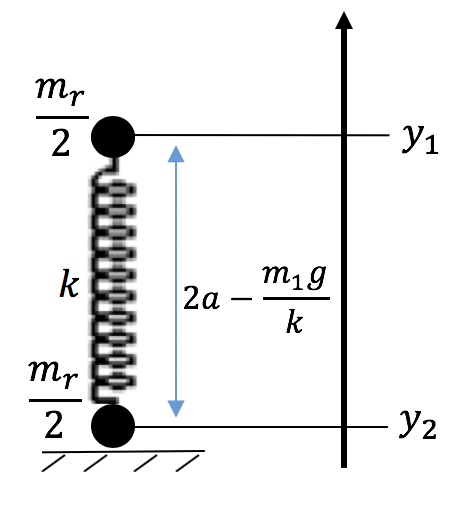
\includegraphics[width=2in]{images_2ddl/repos.png}
\caption{Système au repos}
\label{fig:repos}
\end{figure}

On note $t_0<0$ le moment auquel on relâche le ressort. $t=0$ correspond au moment auquel la masse inférieure quitte le sol, c'est à dire au moment où la force qui lui est transmise par le ressort devient suffisante pour prendre le dessus sur la gravité:$\frac{m_r g}{2}=k(y_1-2a)$. \\
Les positions des masses à $t=0$ sont donc $y_1=2a+\frac{m_r g}{2k}$ et $y_2=0$
On note $t_f$ le temps pour lequel le centre de gravité du système atteint sa hauteur maximale.

\begin{figure}[htb]
\centering
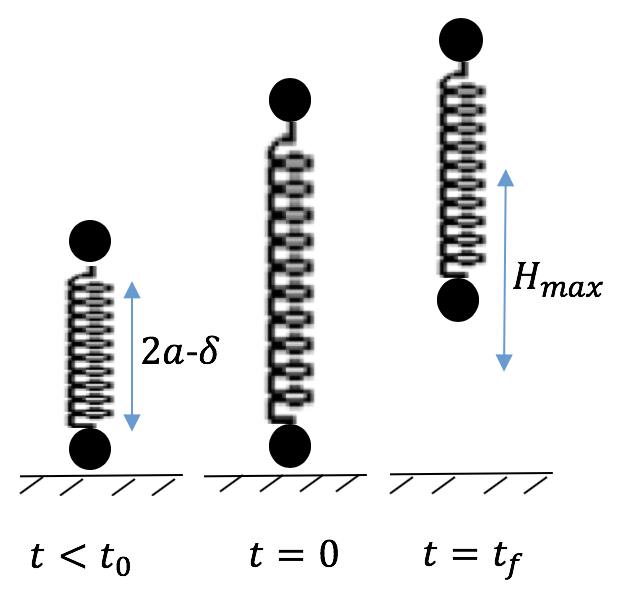
\includegraphics[width=3in]{images_2ddl/saut.png}
\caption{Saut du système}
\label{fig:saut}
\end{figure}

\subsection{Mise en équations}
\begin{equation}
   t_0<t<0: 
  \begin{cases}
    \frac{m_r}{2}\frac{d^2y_1}{dt^2}+k(y_1-2a)+\frac{m_r}{2}g=0\\
    y_2=0
  \end{cases}
  \label{eq:1}
\end{equation}

On pose: $\tau=t-t_0$
Pour $t_0<t<0$, le mouvement est régi par le système suivant:

\begin{equation}
  \begin{cases}
    \tau=t-t_0 \\
    \alpha_0=\sqrt{\frac{2k}{m_r}}\\
    y_1(\tau)=(\frac{m_r g}{2k}-\frac{F}{k})\cos(\alpha_0 \tau)-\frac{m_r g}{2k}+2a \\
    y_2=0
  \end{cases}
  \label{eq:2}
\end{equation}

\begin{equation}
   0<t<t_f: 
  \begin{cases}
    \frac{m_r}{2}\frac{d^2y_1}{dt^2}+k(y_1-y_2-2a)+\frac{m_r}{2}g=0\\
    \frac{m_r}{2}\frac{d^2y_2}{dt^2}+k(y_2-y_1+2a)+\frac{m_r}{2}g=0
  \end{cases}
  \label{eq:3}
\end{equation}

Avec les conditions initiales: 
\begin{equation}
  \begin{cases}
    y_1(0)=2a+\frac{m_r g}{2k}\\
    \frac{d y1}{dt}(0)=v_{10}\\
    y_2(0)=0 \\
    \frac{d y2}{dt}(0)=0
  \end{cases}
  \label{eq:4}
\end{equation}

Le mouvement pour $0<t<t_f$ est décrit par les équations:

\begin{equation}
  \begin{cases}
    \alpha=\sqrt{\frac{4k}{m_r}}\\
    y_1(t)=\frac{1}{2}(-\frac{g t^2}{2}+v_{10}t+(\frac{m_r g}{2k})\cos{\alpha t}+\frac{v_{10}}{\alpha}\sin{\alpha t}+\frac{m_r g}{2k}+4a) \\
    y_2(t)=\frac{1}{2}(-\frac{g t^2}{2}+v_{10}t-(\frac{m_r g}{2k})\cos{\alpha t}-\frac{v_{10}}{\alpha}\sin{\alpha t}+\frac{m_r g}{2k}) 
  \end{cases}
  \label{eq:5}
\end{equation}

Ce qui nous donne les expressions temporelles de la variation de l'allongement du système et de l'évolution de la positon de son centre de gravité:

\begin{equation}
  \begin{cases}
    y_1(t)-y_2(t)= (\frac{m_r g}{2k})\cos{\alpha t}+\frac{v_{10}}{\alpha}\sin{\alpha t}+2a\\
    \frac{y_1(t)+y_2(t)}{2}=\frac{1}{2}(-\frac{g t^2}{2}+v_{10}t+\frac{m_2 g}{k} +2a)
  \end{cases}
  \label{eq:6}
\end{equation}

Ces équations permettent de tracer des animations du mouvement afin de mieux appréhender ce dernier par la suite. Tout au long de l'élévation du centre de gravité de la roue, on peut observer des déformations correspondant au second mode vibratoire d'un anneau (déformations planes).
\\ 
\\
Bilan d'énergie appliqué au système {masse 1 + masse 2 + ressort}
\begin{itemize}
    \item On prend pour référence de l'énergie potentielle la position du système à l'équilibre statique: $y_{1,ref}=2a-\frac{m_r g}{2k}$ et $y_{2,ref}=0$.
    \item $t<t_0$: $E=\frac{F^2}{2k}$
    \item $t=0$ : $E=\frac{1}{4}m_r v_{10}^2 +\frac{5}{8}\frac{(m_r g)^2}{k} $
\end{itemize}

On en déduit l'expression de la vitesse de la masse 1 à $t=0$: $v_{10}=\sqrt{\frac{2(F^2-\frac{5(m_r g)^2}{4})}{m_r k}}$ \\

Lorsqu'on arrive à $t=t_f$, la vitesse du centre de gravité s'annule. Il suffit alors de dériver l'expression de la position du centre de gravité déterminée ci-dessus pour obtenir: $t_f=\frac{v_{10}}{g}$, soit: 
$$ =\sqrt{\frac{2(F^2-\frac{5(m_r g)^2}{4})}{m_r k g^2}}$$

On substitue ensuite cette expression à $t_f$ dans l'expression de la position du centre de gravité pour svoir la hauteur maximale de ce dernier, à laquelle on soustrait $y_{1,ref}$ pour obtenir finalement l'expression de $H_{max}$.
\\ \\
Ainsi: $H_{max}=\frac{1}{2}(\frac{F^2}{m_r k g}-\frac{0.25m_r g}{k})$
\\
Ou encore, en fonction de la pulsation propre $\alpha$: $H_{max}=\frac{1}{2}(\frac{4F^2}{m_r^2\alpha^2 g}-\frac{g}{\alpha^2})$.
\\ \\
Ainsi, les paramètres influençant la hauteur maximale de saut du système sont:
\begin{itemize}
    \item La force de compression $F$ à laquelle ce dernier est soumis initialement
    \item La masse du système, déterminée par sa géométrie et la masse volumique du matériau
    \item La raideur équivalente du système qui dépend de sa géométrie et du module de Young du matériau.
\end{itemize}

L'expression de $H_{max}$ nous permet d'étudier l'efficacité énergétique du système, c'est à dire d'estimer quelle fraction de l'énergie totale fournie au système sous forme de déformation élastique est convertie en énergie potentielle gravitationnelle servant au saut. \\
Pour cela on s'intéresse au ratio $\frac{E_{p,g}}{E_{tot}}$ des deux quantités décrites précedemment. \\
Avec $E_{tot}=\frac{F^2}{2k}$ et $E_{p,g}=m_r g H_max$, on obtient:  $\frac{E_{p,g}}{E_{tot}}=1-\frac{(m_r g)^2)}{4F^2}$.

\subsection{Traitement numérique du modèle}
Dans la partie qui suit, on étudie pour chaque paramètre dont dépendent $H_max$ et le ratio d'efficacité énergétique comment ces derniers évoluent lorsqu'on fait varier un de ces paramètre indépendamment des autres.
\\ 
\\ 
La variation de ces paramètres doit respecter les valeurs limites suivantes, en dessous desquelles le modèle n'est plus valide:
\begin{itemize}
    \item Pour $F$: Pour que le modèle soit valide il faut qu’il y ait un saut, l'énergie de déformation élastique doit être suffisante pour faire décoller la masse 2, ce qui se traduit par: $\frac{1}{2} \frac{F^2}{k}>\frac{(m_r g)^2}{4k}$  soit: $F>\frac{m_r g}{/sqrt{2}}$
    \item Pour $k$: Le ressort doit pouvoir soutenir la masse 1: $\frac{m_r g}{2k}<2a$ c'est à dire: $k>\frac{m_r g}{4a}$ 
    \item Pour $m_r$: Diminuer $m_r$ revient à retirer de la matière, il y a donc une masse limite dépendant des propriétés mécaniques du matériau en dessous de laquelle il y aura rupture lors de la compression, la roue étant devenue trop fragile.
\end{itemize}
Les limites seront indiquées par des pointillés sur les tracés plus bas
\\
On applique le modèle développé dans la section précédente aux quatre cas suivants:
\begin{itemize}
	\item Une roue en acier dont les dimensions, détaillées en Figure~\ref{fig:geo1} ,  ont été mesurées sur une roue existante (cas témoin)
	\item Une roue en matériau composite de dimensions identiques à celles de la première
	\item Une roue en matériau composite de section elliptique dont le prolongement du petit axe coincide avec l'axe de révolution (cas 1), dont les dimensions sont détaillés Figure~\ref{fig:geo2}
	\item Une roue en matériau composite de section elliptique dont le prolongement du grand axe coincide avec l'axe de révolution (cas 2), dont les dimensions sont détaillés Figure~\ref{fig:geo2}
\end{itemize}

\begin{figure}[htb]
\centering
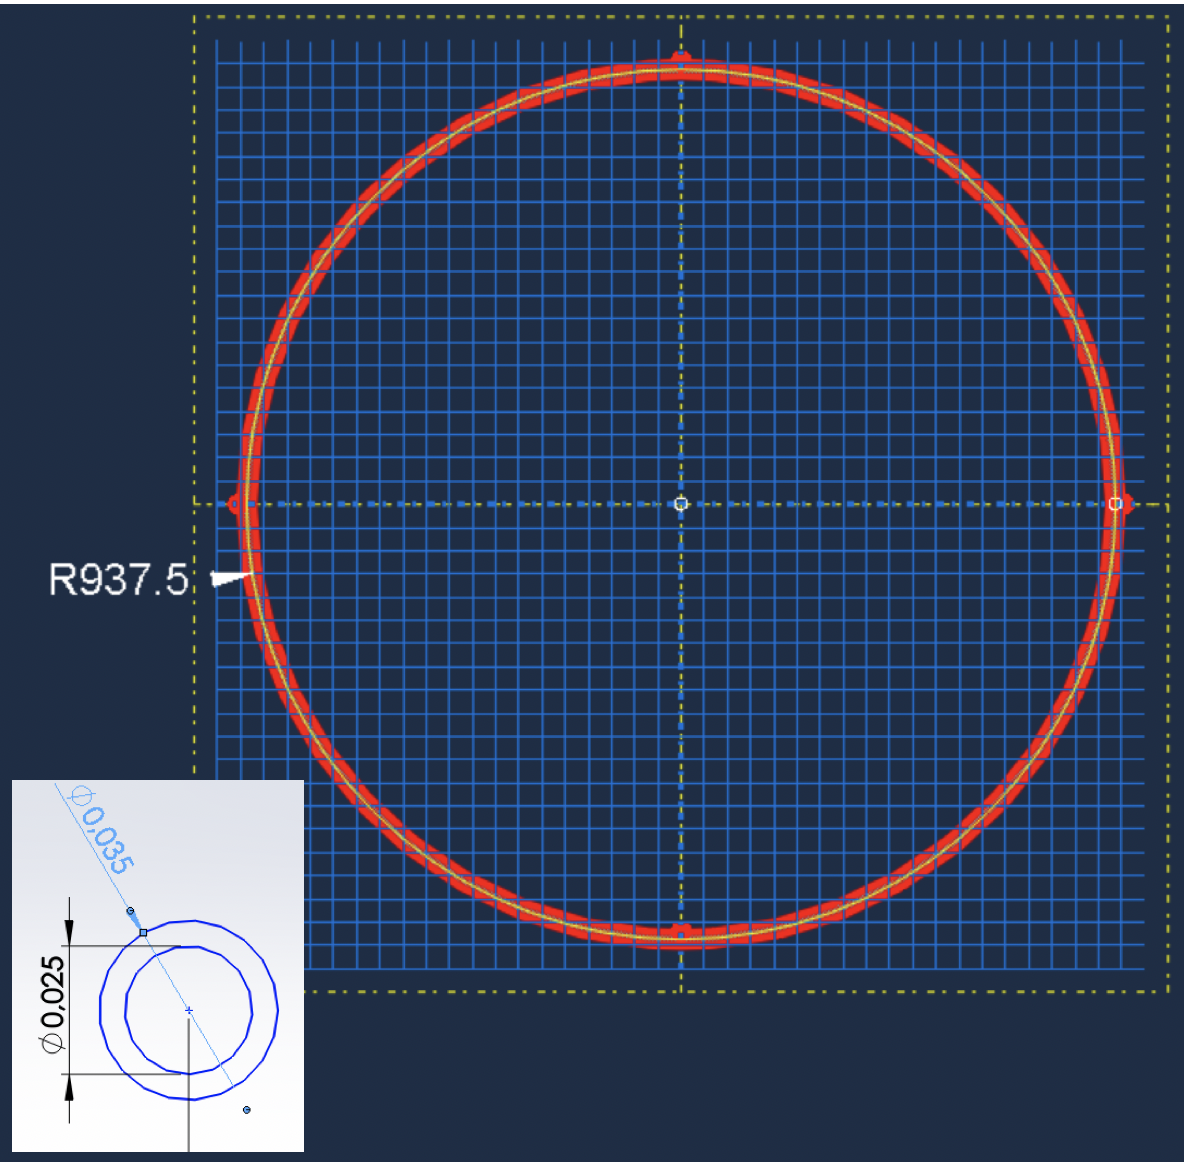
\includegraphics[width=4in]{images_2ddl/geo1.png}
\caption{Géométrie et dimension des roues Cyr à sections circulaires étudiées dans cette partie}
\label{fig:geo1}
\end{figure}

\begin{figure}[htb]
\centering
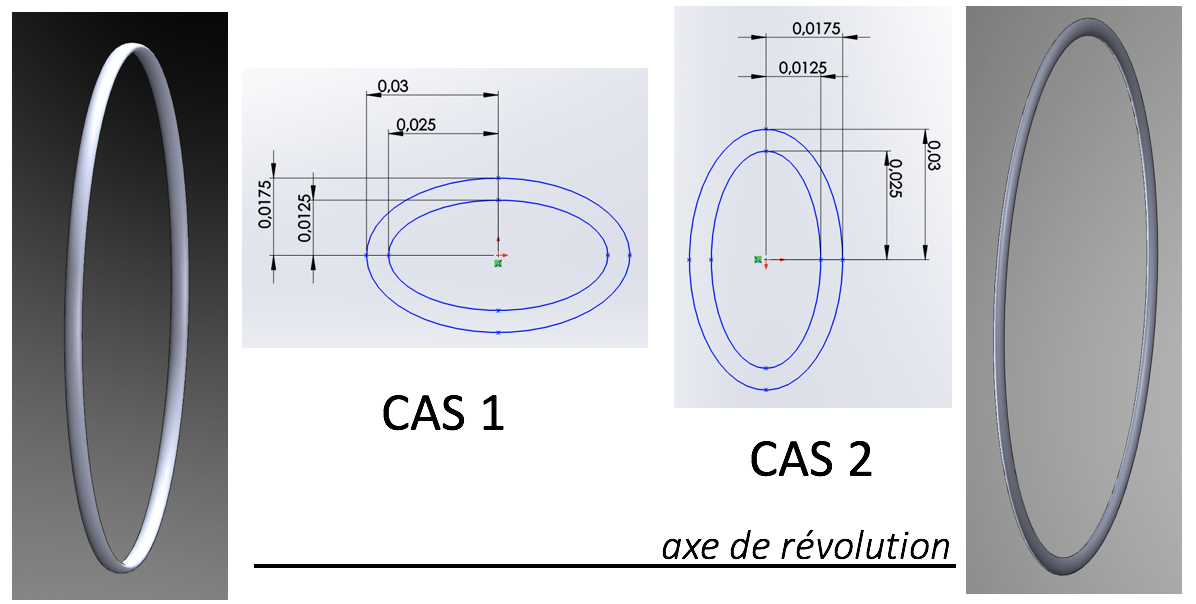
\includegraphics[width=4in]{images_2ddl/geo2.png}
\caption{Géométrie et dimension des roues Cyr à sections elliptiques étudiées dans cette partie}
\label{fig:geo2}
\end{figure}


Si on fait varier un paramètre indépendamment des autres, il est nécessaire d'affecter une valeur à ces derniers, fixés momentanément:
\begin{itemize}
	\item Les géométries considérées sont celles présentées en  Figures \ref{fig:geo1} et \ref{fig:geo2}
	\item On considère que la force $F$ appliquée au système a pour norme $900 N$, correspondant au poids d'un athlète se suspendant à une main à la roue.
	\item Les propriétés mécaniques de l'acier sont les suivantes $E_a=210GPa$, $rho_a=7800 kg m^-3$
	\item Pour le matériau composite, on considère dans un premier temps qu'il s'agit d'une matrice nylon renforcée de fibres de carbones courtes, qu'on considère isotrope. On a donc: $E_c=9 GPa$, $G=3.8 GPa$, $rho_c=1170 kg m^-3$, avec une contrainte à la rupture $\sigma_r=63 MPa$
\end{itemize}
Dans ce qui suit, lorsqu'on fait varier une seul paramètre, les autres, momentanément fixés, prennent les valeurs qui leur ont été attribuées ci-dessus.
\\
\\ 
Premièrement, avec ces données il est possible de déterminer la masse minimale que devra avoir la roue (on considère le cas d'une section circulaire):
\begin{itemize}
    \item On commence par calculer les contraintes lorsque la roue est comprimée par une force $F$: La contrainte dans l'arrête extérieure s'exprime $\sigma_i=k_i\sigma$ \cite{roark},
    où sigma est la contrainte calculée pour une poutre droite: $\sigma=\frac{Mr_2}{I_z}$, avec $I_z=\frac{\pi}{2}(r_2^4-r_1^4)$ et $M=\frac{\pi}{4}FR$.
    D'après les formules du livre de Roark, $k_i$ s'exprime $k_i=\frac{1}{4\beta}\frac{1-\beta}{\frac{R_c}{r_2}-1}[1+(\frac{r_1}{r_2})^2]$ avec $\beta=\frac{1}{2}[\frac{2R_c}{r_2}-\sqrt{(\frac{R_c}{r_2})^2-1}-\sqrt{(\frac{R_c}{r_2})^2-(\frac{r_1}{r_2})^2}]$ 
    \item Il ne reste plus qu'à déterminer le rayon de courbure de la roue comprimée, comme illustré sur la figure \ref{fig:ellr}: $R_c=\frac{a_r^2}{b_r}$, $a_r$ et $b_r$ étant respectivement les demi grand axe et demi petit axe de l'ellipse que devient la roue lorsqu'elle est comprimée.\\
    
    \begin{figure}[htb]
    \centering
    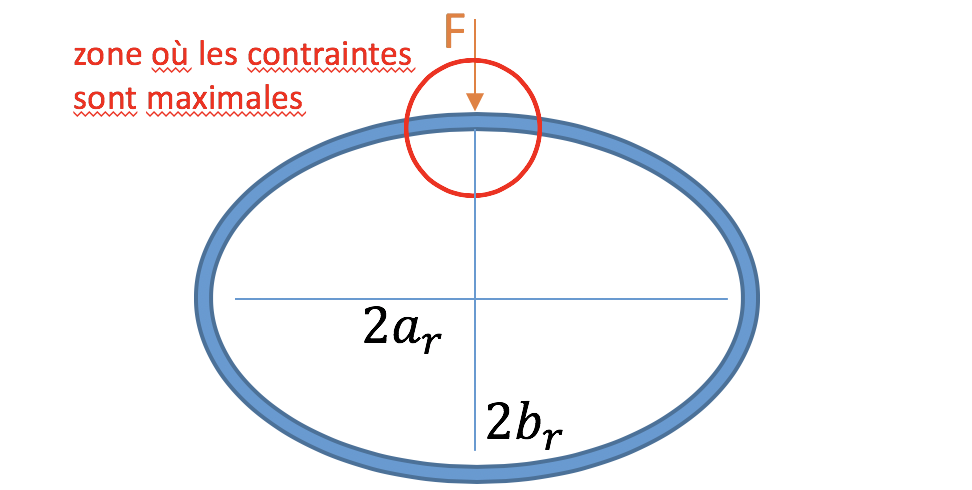
\includegraphics[width=4in]{images_2ddl/ellr.png}
    \caption{}
    \label{fig:ellr}
    \end{figure}
    
\begin{itemize}
    \item Pour calculer $a_r$ et $b_r$, on utilise les formules du livre de Roark qui donnent les variations de diamètre horizontal $\Delta D_h$ et vertical $\Delta D_v$ d'une anneau comprimé selon son diamètre avec une force $F$, et on aura ainsi $a_r=R+\frac{\Delta D_h}{2}$ et $b_r=R+\frac{\Delta D_v}{2}$.
    \item D'après les formules de Roark, $\Delta D_h=\frac{FR^3}{EI}(\frac{1}{2}(1+\frac{I}{AR^2}+\frac{2EI}{GAR^2})-1+\frac{2}{/pi}(1-\frac{I}{AR^2})^2)$ et $\Delta D_v=-\frac{FR^3}{EI}(\frac{\pi}{4}(1-\frac{I}{AR^2}+\frac{2EI}{GAR^2})-\frac{2}{/pi}(1-\frac{I}{AR^2})^2)$, où $A$ est l'aire de section, $E$, le module de Young, $G$, le module de cisaillement, $R$, le rayon médian de la roue, et $I$ le moment de section quadratique selon l'axe principal perpendiculaire au plan de la roue.
    \item En implémentant numériquement les équations ci-dessus, on est capable de calculer les contraintes maximales auxquelles sera soumise la roue pour une force de compression $F$ donnée. Pour $F=900N$, en fixant $r_2$ et en faisant varier $r_1$ de $0$ à $r_2$, on est capable de tracer les contraintes maximales, en fonction de la masse de la roue, $m_r=2\pi\rho A R$. Comme l'illustre la figure-\ref{fig:mmin1} ci-dessous, il est alors possible de déterminer la masse à partir de laquelle les contraintes passent sous le seuil de $63 MPa$, et donc à partir de laquelle il y a rupture.
    
\end{itemize}


\begin{figure}[htb]
\centering
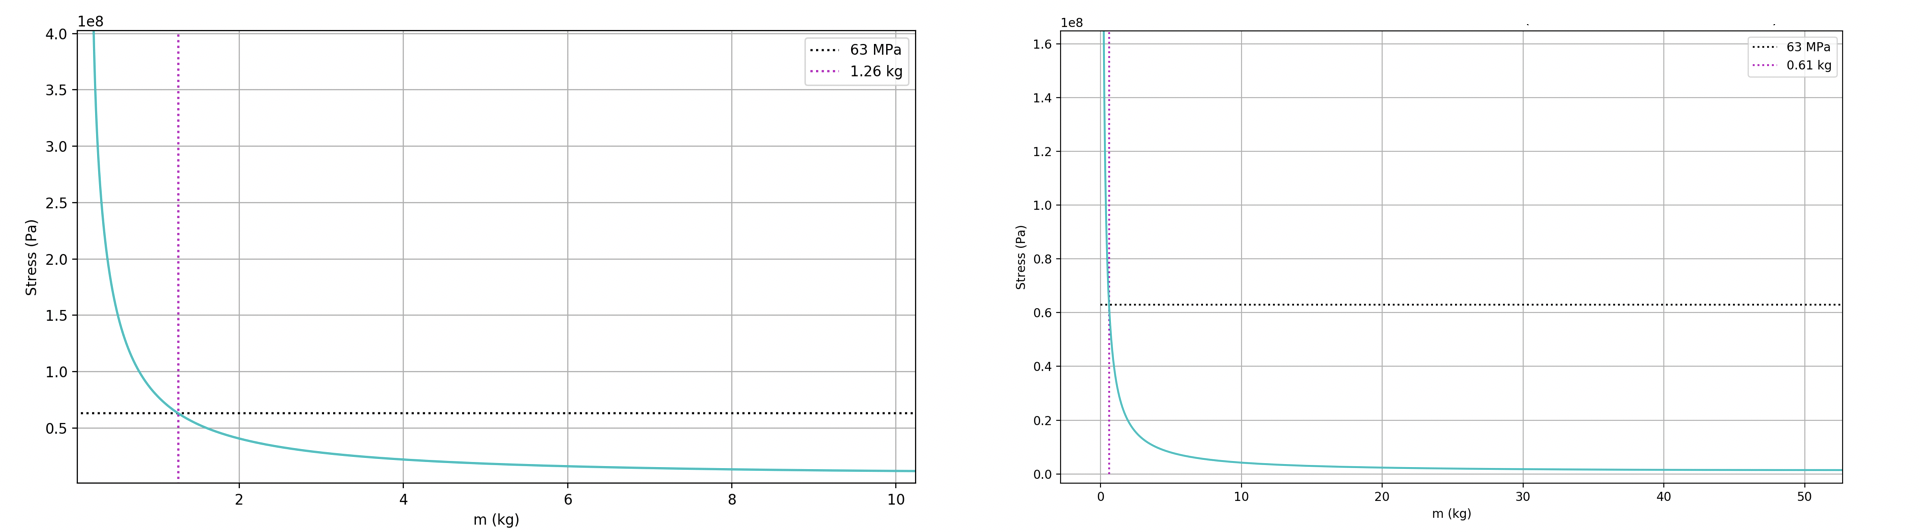
\includegraphics[width=7in]{images_2ddl/mmin1.png}
\caption{Contraintes maximales dans la roue en fonction de sa masse, pour $r_2=2.5 cm$ et $r_1$ variant de $0.0$ à $2.49 cm$ (gauche) et $r_2=5.0 cm$ et $r_1$ variant de $0.0$ à $4.99 cm$}
\label{fig:mmin1}
\end{figure}


\begin{itemize}
    \item On peut donc implémenter ce procédé numériquement pour déterminer cette valeur minimale de la masse pour en fonction de $r_2$. Le resultat de l'implémentation est présenté à la figure-\ref{fig:mmin2} ci-dessous. 
\end{itemize}


\begin{figure}[htb]
\centering
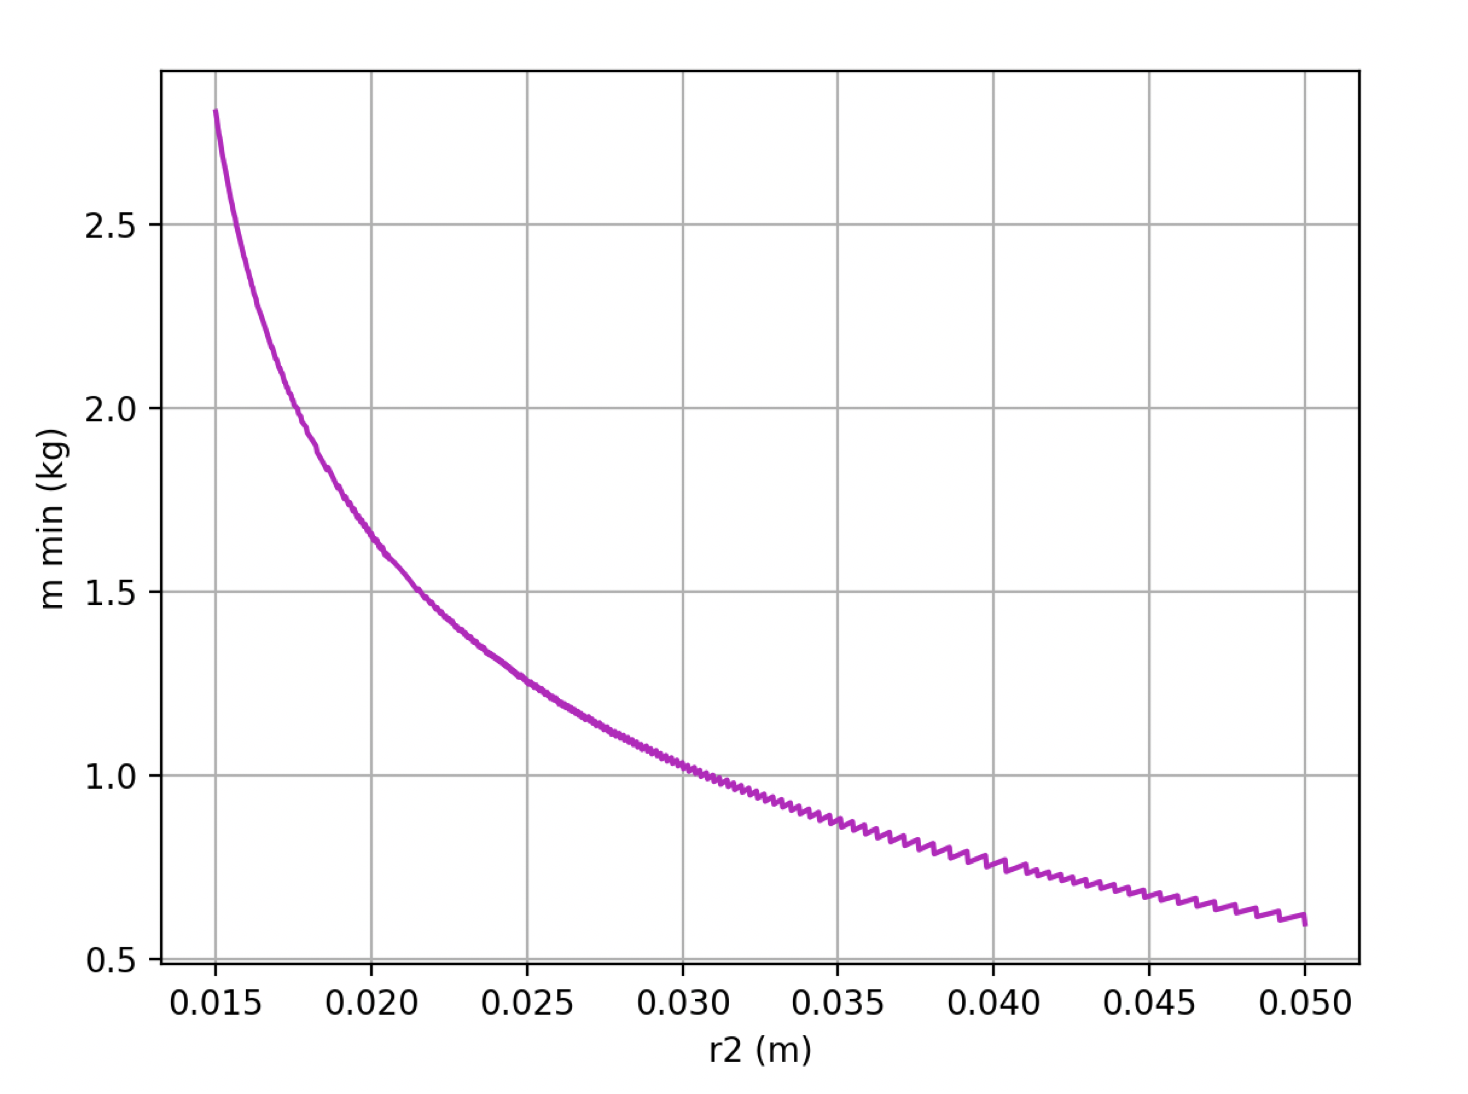
\includegraphics[width=4in]{images_2ddl/mmin2.png}
\caption{Masse minimale de la roue en fonction de $r_2$}
\label{fig:mmin2}
\end{figure}


\item Pour ce qui suit, $r_2$ sera fixé à $1.75 cm$, la masse minimale sera donc $2.0 kg$

\end{itemize}

\begin{figure}

  \begin{subfigure}
  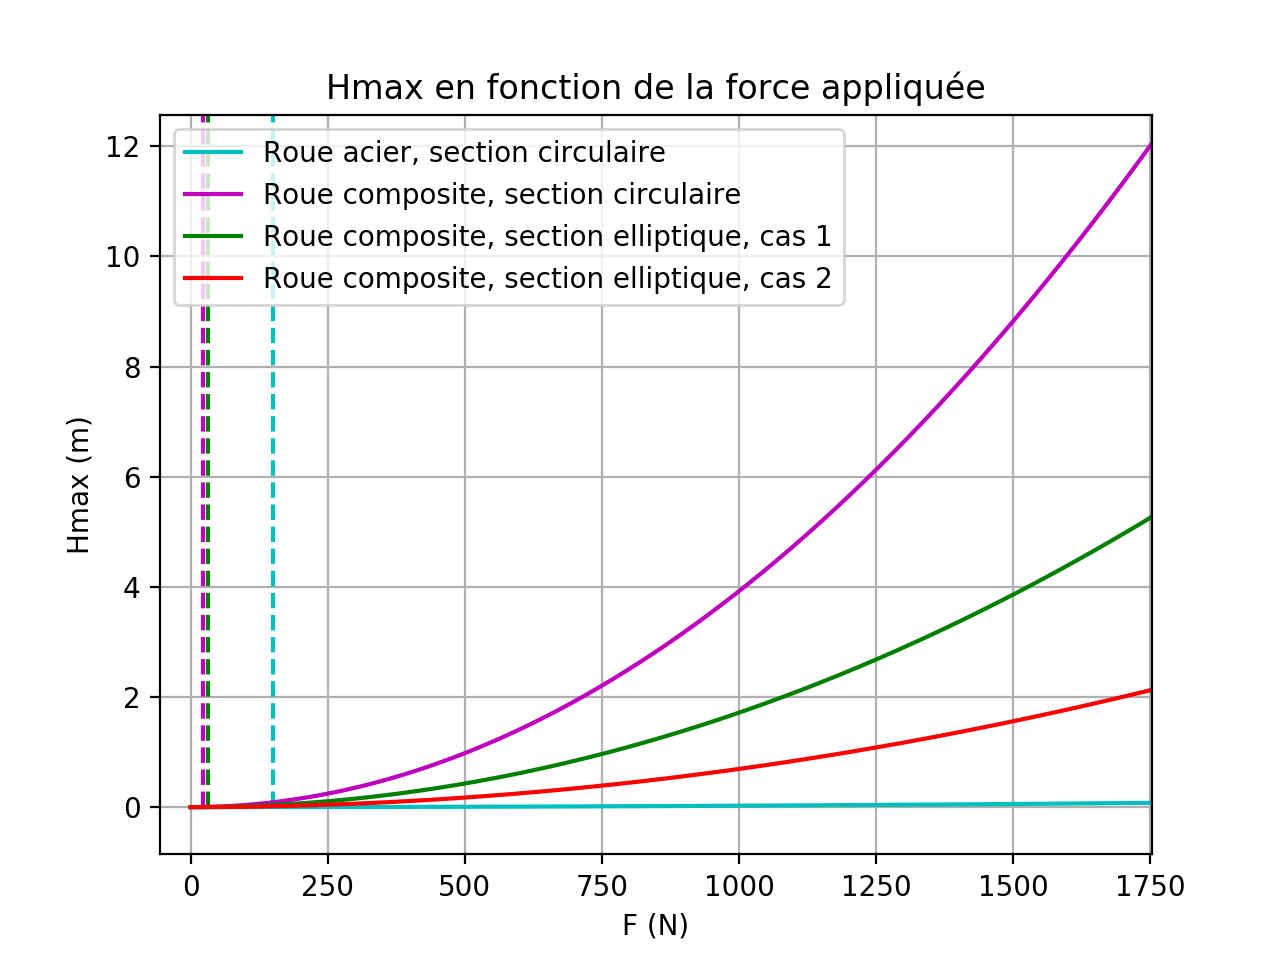
\includegraphics[width=3in]{images_2ddl/hmaxf.png}
  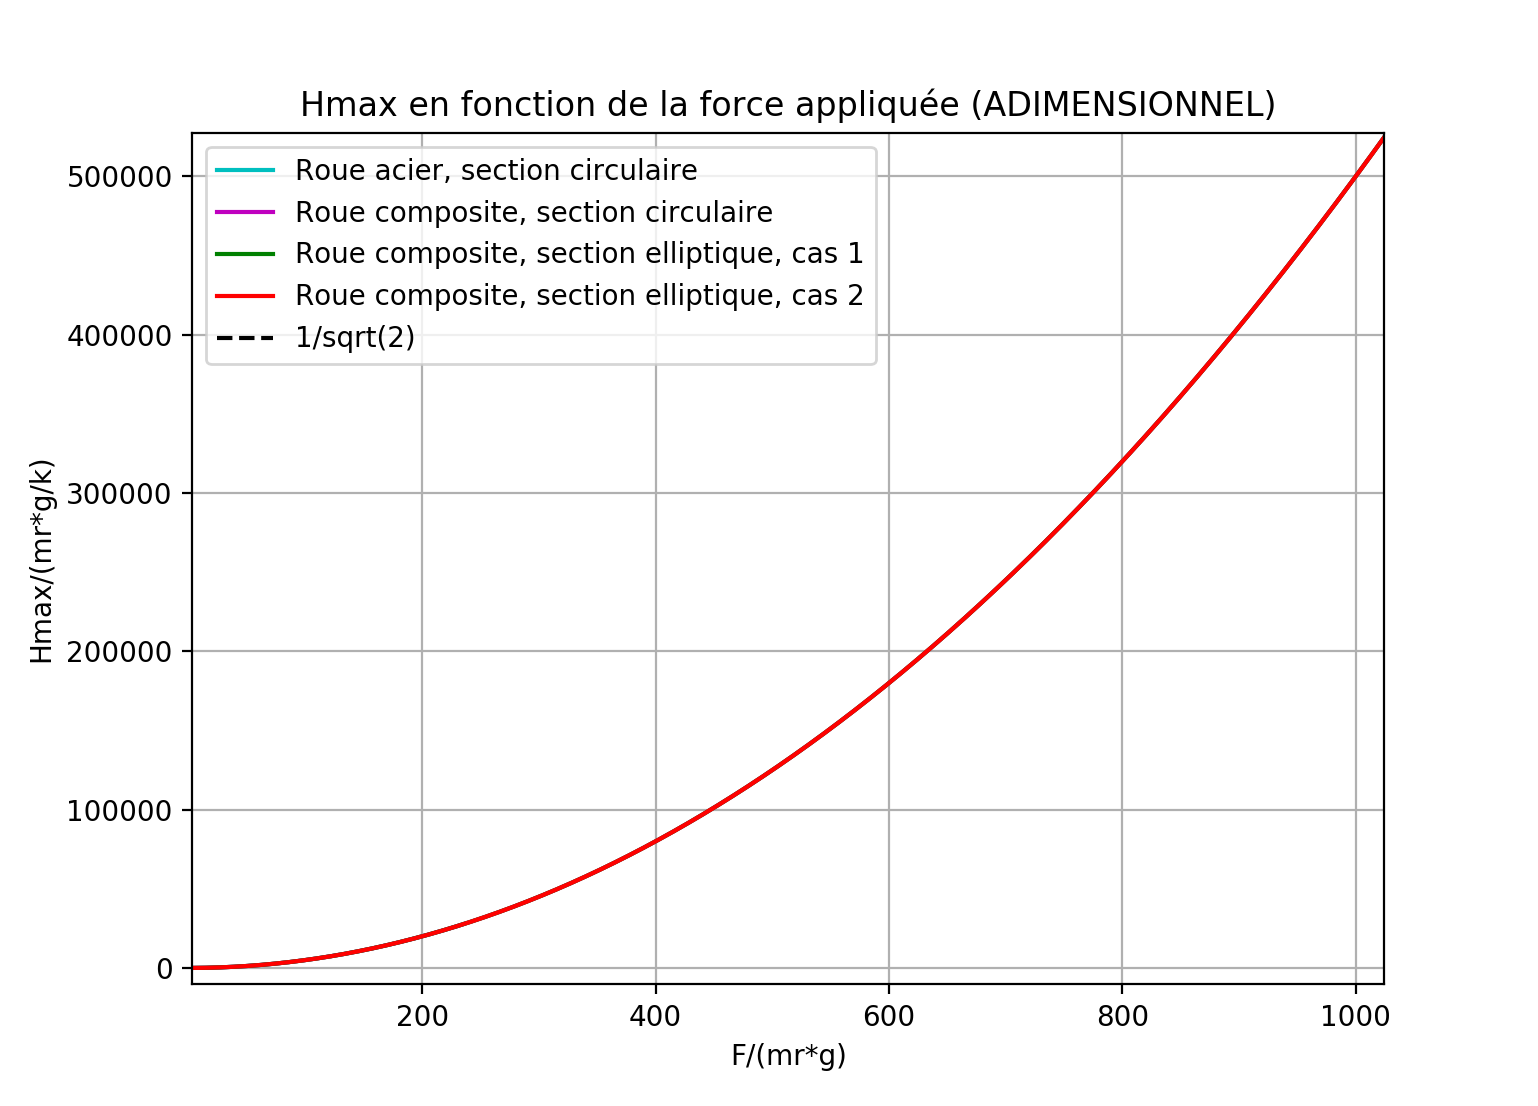
\includegraphics[width=3in]{images_2ddl/hmaxfa.png}
  \end{subfigure}
  \begin{subfigure}
  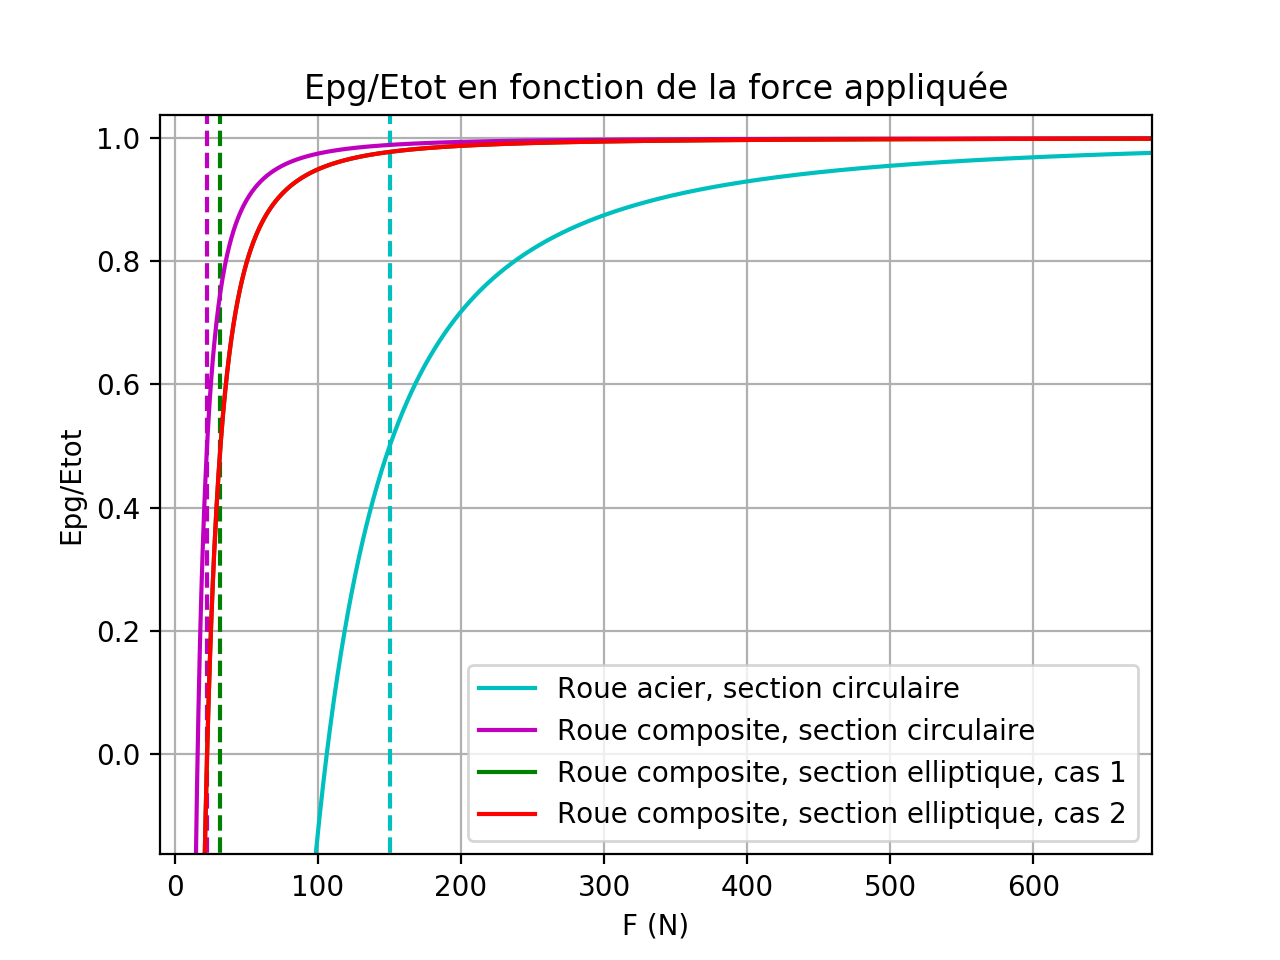
\includegraphics[width=3in]{images_2ddl/epf.png}
  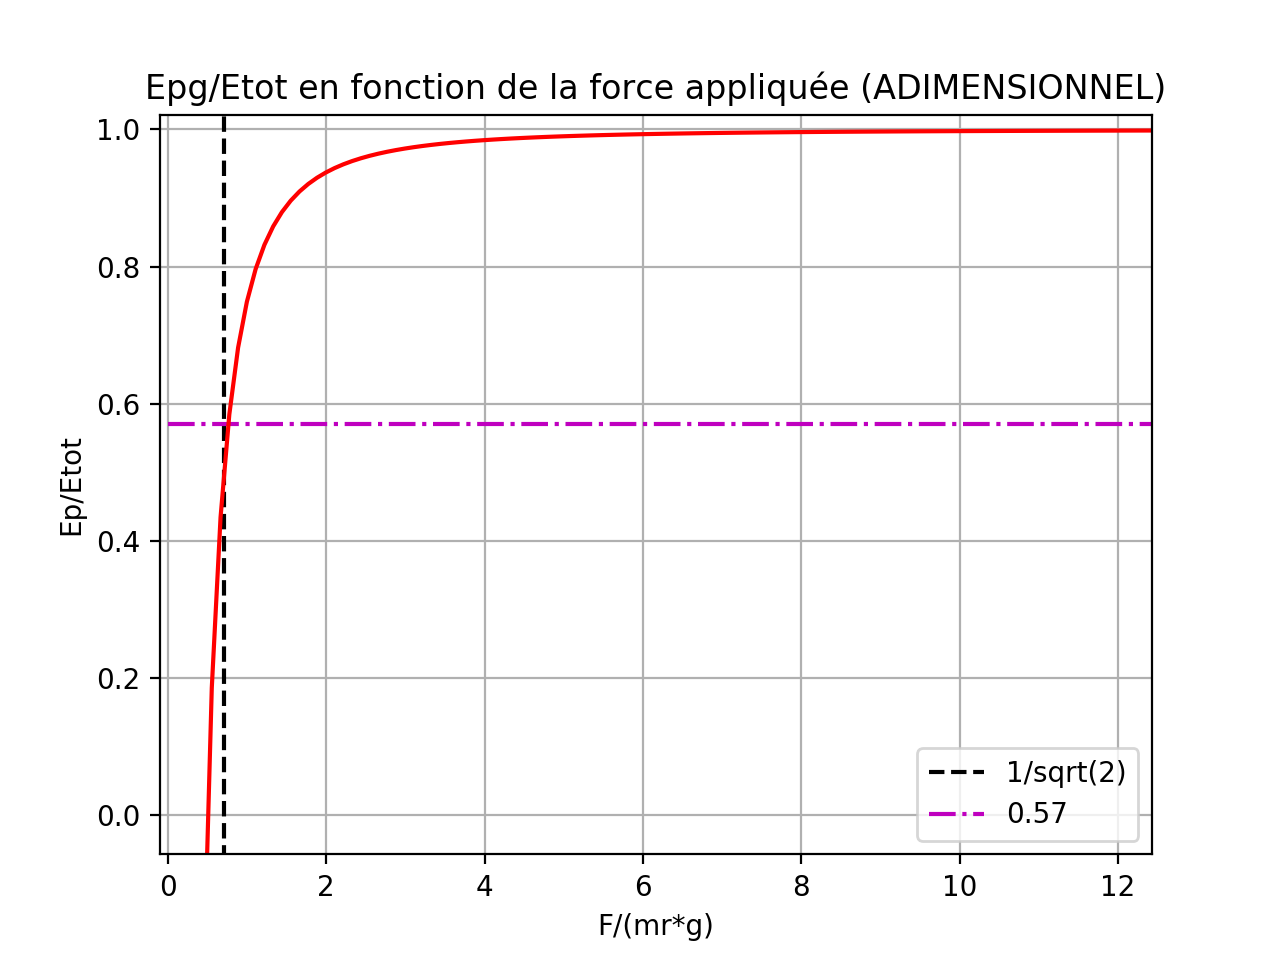
\includegraphics[width=3in]{images_2ddl/epfa.png}
  \end{subfigure}
  \begin{subfigure}
  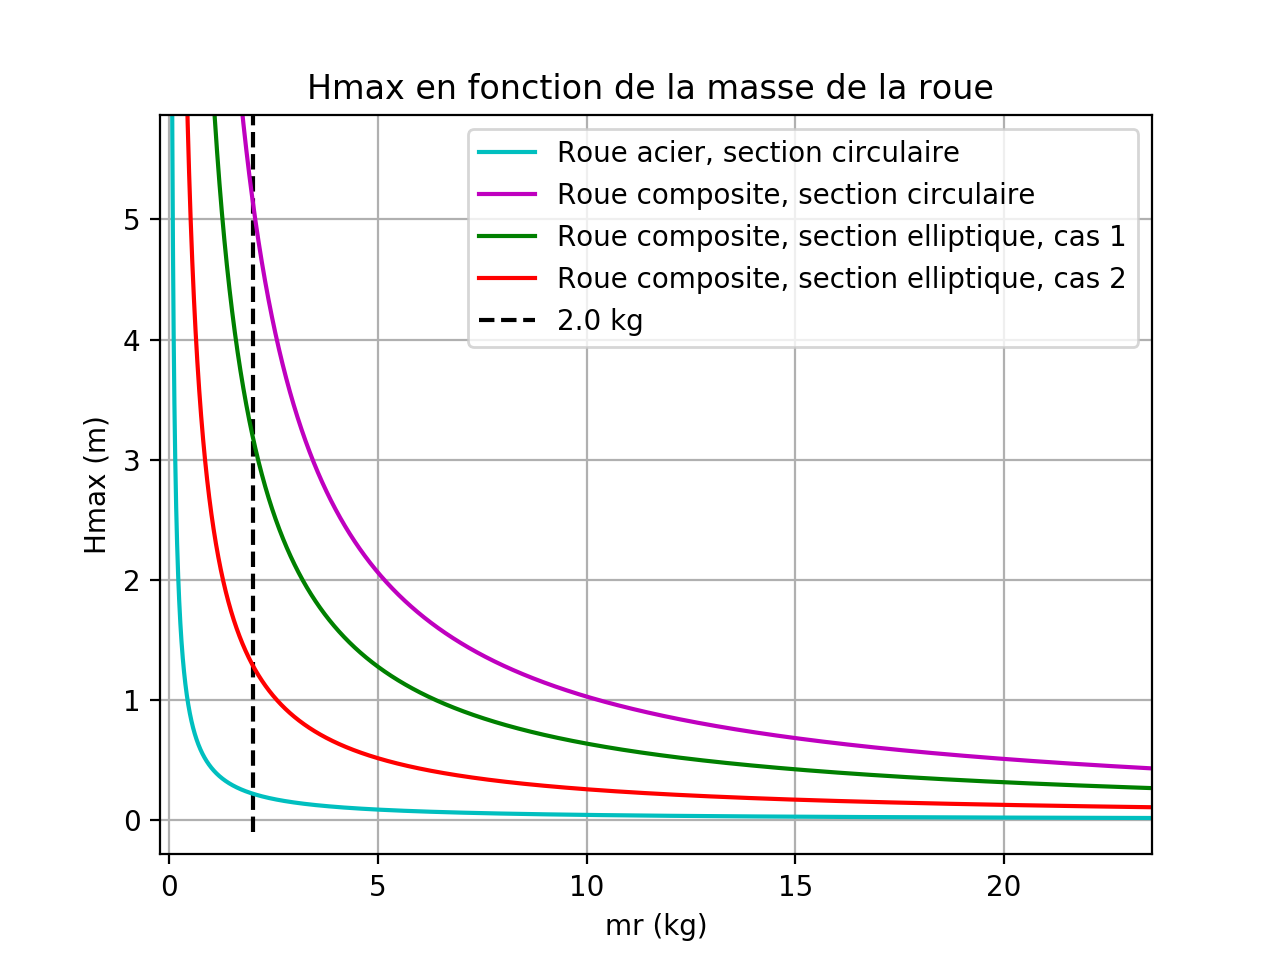
\includegraphics[width=3in]{images_2ddl/hmaxm.png}
  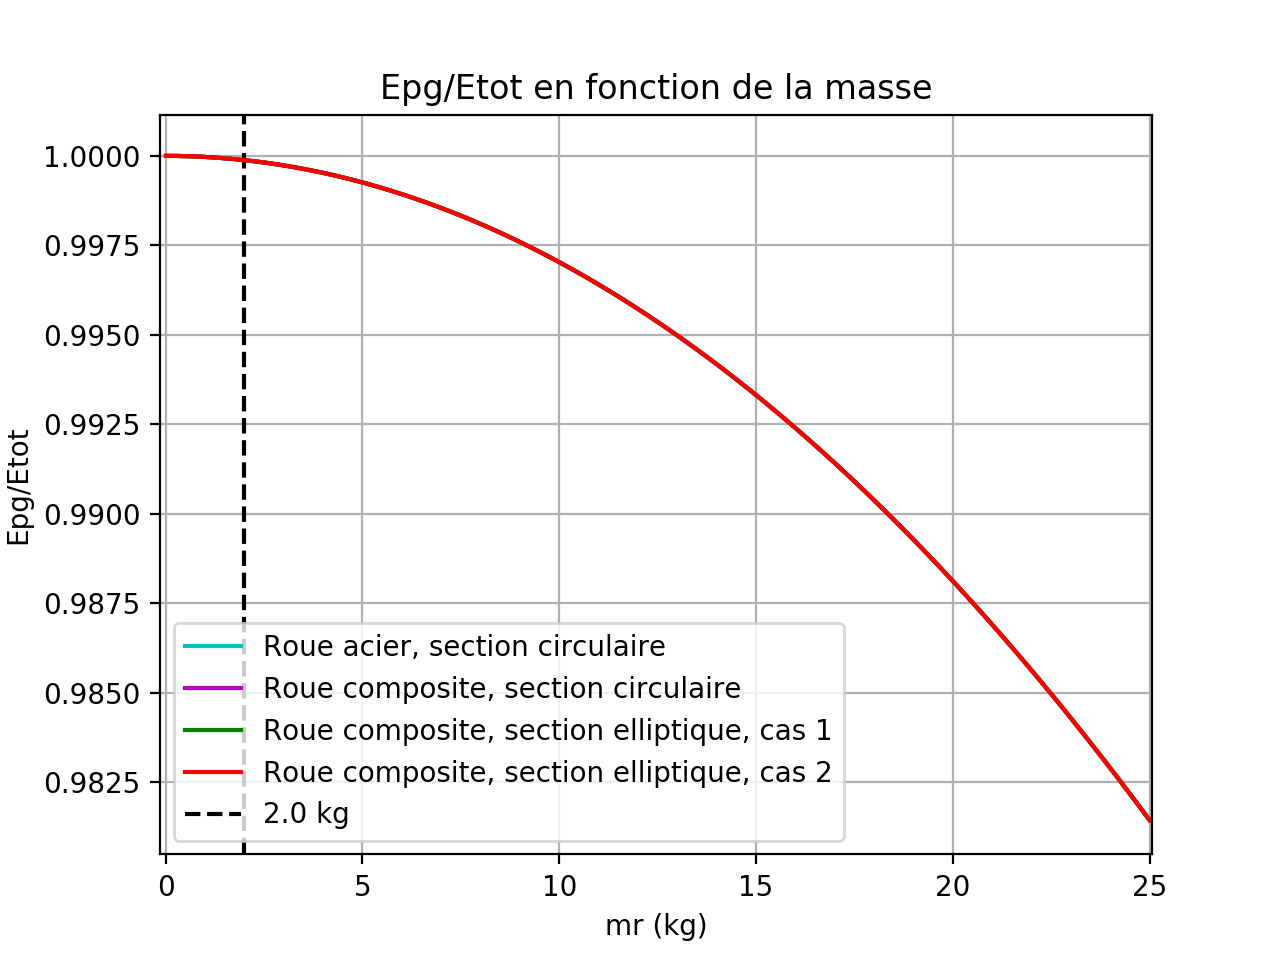
\includegraphics[width=3in]{images_2ddl/epm.png}
  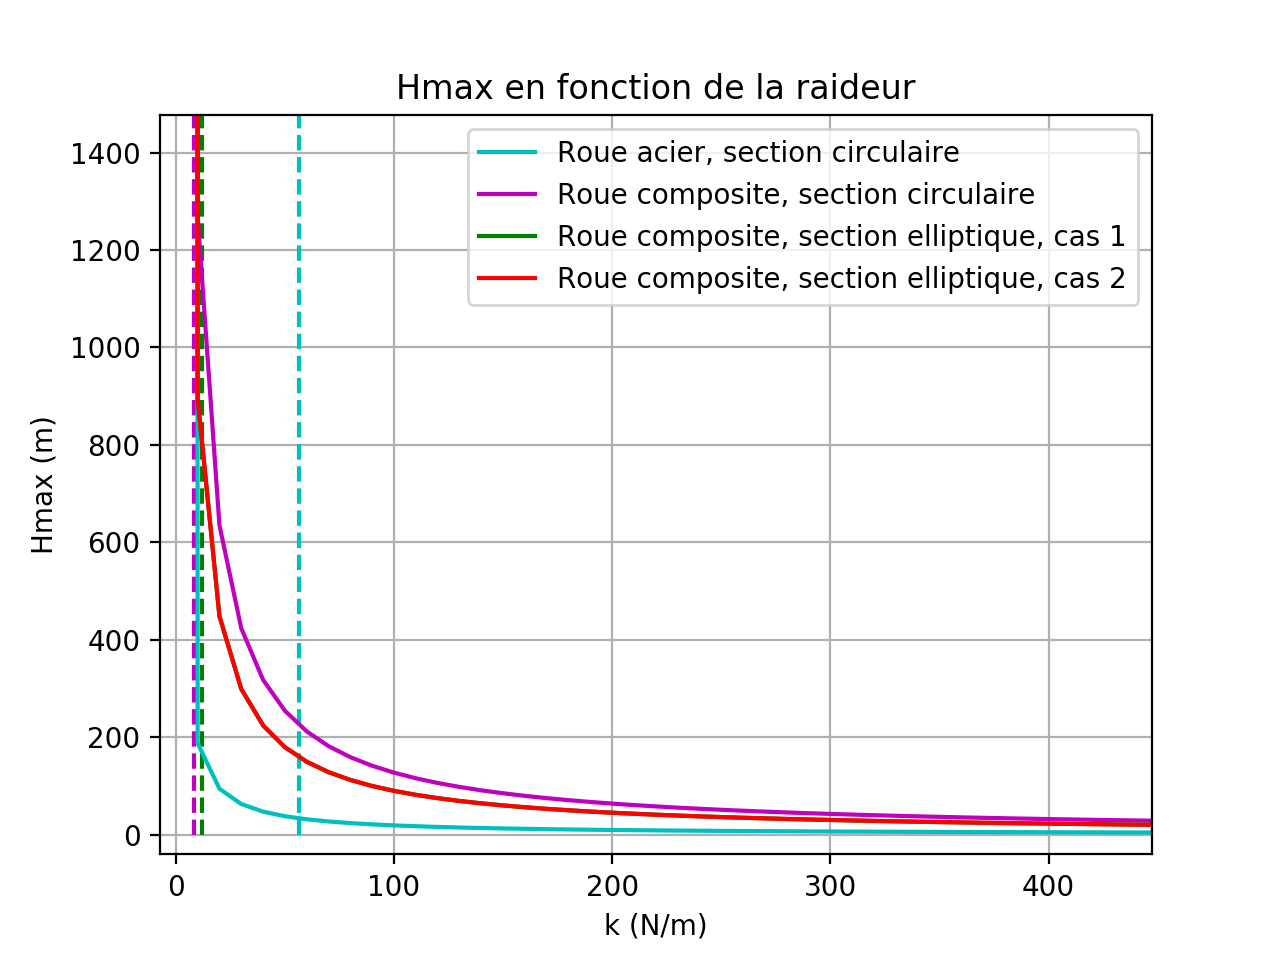
\includegraphics[width=3in]{images_2ddl/hmaxk.png}
  \end{subfigure}
  
  \caption{Variations de $H_{max}$ et de $\frac{E_{p,g}}{E{tot}}$}
\end{figure}



Remarques:
\begin{itemize}
    \item Les tracés adimensionnels permettent d'étudier une tendance globale, ainsi que de s'affranchir de la dépendance des résultats avec les autres paramètres.
    \item Le rendement énergétique minimal est 0.57, lorsque $F$ est égale à sa valeur limite
    \item Pour les roues composites définies plus haut, et le modèle étudié présentement, le rendement énergétique avoisine les 100\% à partir d'une certaine force ($F=200 N$ dans notre cas )
    \item Une variation de la masse influe peu sur l'efficacité énergétique, qui reste élevée sur la figure \ref{fig:epm}, tracée pour une force $F=900 N$. La force appliquée à la roue est le paramètre déterminant pour cette dernière. Dans la continuité de cette observation, l'accentuation de la pente, croissante avec la force, traduit une "rentabilité" de l'énergie d'autant meilleure que la force qu'on applique est élevée.
    \item A l'inverse, la courbe $H_{max}=f(k)$ s'aplatit rapidement à mesure que la raideur augmente. Il s'agit de trouver un compromis entre la solidité et la maximisation de la hauteur de saut.
\end{itemize}


\section{Stabilité dynamique du mouvement}
\subsection{Description du mouvement}
On étudie ici le second mouvement caractéristique de la roue Cyr, analogue au mouvement du disque d'Euler. Le mouvement se découpe en deux phases, une première phase au cours de laquelle la roue décrit des cercles en roulant sur sa tranche, puis une deuxième phase où elle oscille en tournant de plus en plus vite avant de tomber à plat, stoppant net le mouvement. Ces deux phases correspondent à l'énchainement de deux figures de roue Cyr, la "roue" pour la phase 1 et la pièce pour la phase 2. \\
Ce qui suit est basé sur l'article de Batista \cite{Batista}, dont la démarche et le modèle mathématique développés pour le disque d'Euler ont été adaptés à la géométrie torique de la roue Cyr. De même que Batista, l'objectif est de développer des cartes de stabilité dynamiques, avec d'autres variables adaptées à notre cas.

\subsection{Hypothèses}
\begin{itemize}
    \item On se place en régime stationnaire: les variables qui prennent ainsi des valeurs constantes seront indicées d'un 0.
    \item On considère que la roue évolue sur un sol rugueux: il n'y a pas de glissement au niveau du point de contact.
    \item Le mouvement est étudié pour des valeurs de $\theta_0$ strictement comprises entre 0 et $\pi/2$ radians.
\end{itemize}

\subsection{Mise en équations}
\subsubsection{Variables et systèmes de coordonnées}

\begin{table}[htbp]
  \centering
  \caption{Constantes et variables des modèle analytiques}
  \begin{tabular}{|c|l|}
    \hline\rowcolor[gray]{0.8}\color{black}
    Symbole         & Description\\\hline
    $C$             & Centre de gravité de la roue\\\hline
    $P$             & Point de contact entre la roue et le sol\\\hline
    $A$             & Point autour duquel la roue roule en dessinant des cercles\\\hline
    $a$             & Rayon externe de la roue\\\hline
    $R$             & Rayon médian de la roue\\\hline
    $r_c$             & Rayon des cercles dessinés par la roue, obtenus par projection du centre de masse au sol\\\hline
    $(X_C,Y_C,Z_C)$           & Position du centre de gravité dans le reférentiel OXYZ\\\hline
    $(\psi,\theta,\phi)$       & Position angulaire de la roue dans OXYZ\\\hline
    $(v_{Cx},v_{Cy},v_{Cz})$           & Composantes de la vitesse du point C dans C{xzy} \\\hline
    $(\omega_1,\omega_2,\omega_3)$          & Composantes de la vitesse angulaire $\vec{omega}$ dans $C{\xi \eta \zeta}$\\\hline
    $\Omega$          & Vitesse angulaire par rapport à l'axe Z\\\hline
    $(F_x,F_y,F_z)$          & Composante de la force de réaction au point $P$ dans $C_{xzy}$ \\\hline
    $(M_x,M_y,M_z)$          & Composante du moment de réaction au point $P$ dans $C_{xzy}$ \\\hline
    $\Omega$          & Vitesse angulaire par rapport à l'axe Z\\\hline
  \end{tabular}
  \label{tab:batista}
\end{table}

On reprend les trois référentiels utilisés par Batista: $OXYZ$, $C{xzy}$ et $C{\xi\eta\zeta}$:

\begin{figure}[htb]
\centering
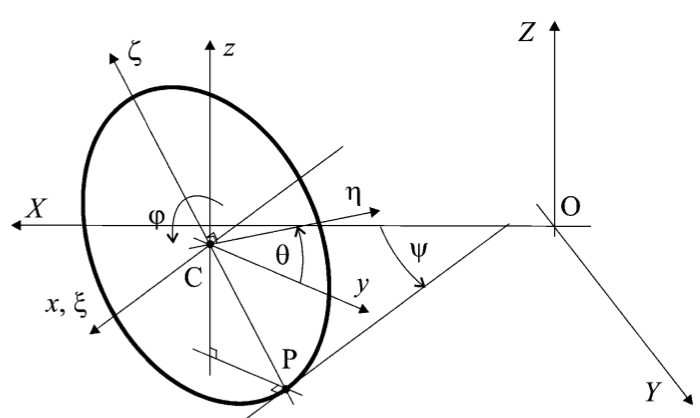
\includegraphics[width=4in]{batista/ref1.png}
\caption{Système de coordonnés, tiré de l'article de Batista \cite{Batista}}
\label{fig:ref1}
\end{figure}

\begin{figure}[htb]
\centering
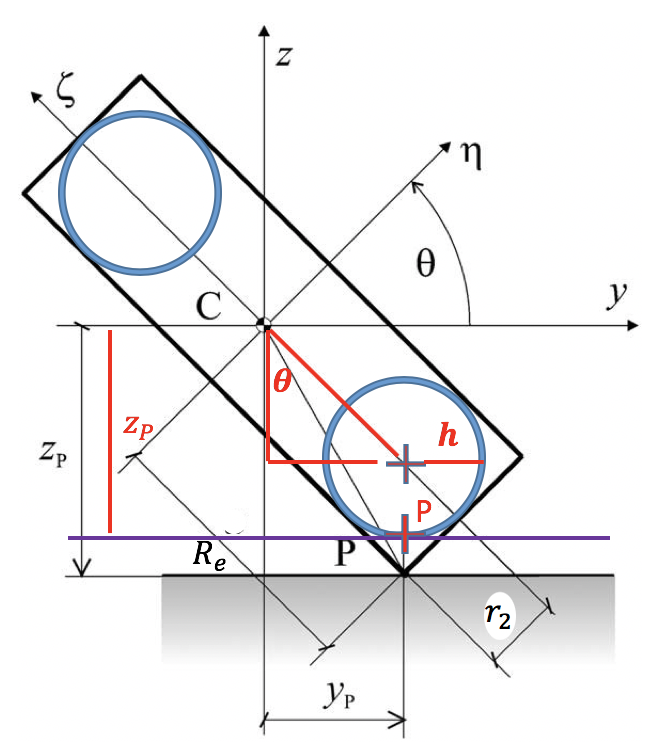
\includegraphics[width=4in]{batista/ref2.png}
\caption{Système de coordonnés, adapté de l'article de Batista \cite{Batista}}
\label{fig:ref2}
\end{figure}

\subsubsection{Equations}
Le mouvement de la roue est régie par les équations cinématiques suivantes \cite{Batista}:
\begin{equation}
  \begin{cases}
    \frac{dX_C}{dt}=v_{Cx0} \cos{\psi}- v_{Cy0} \sin{\psi}\\
    \frac{dY_C}{dt}=v_{Cx0} \sin{\psi}- v_{Cy0} \cos{\psi}\\
    \frac{dZ_C}{dt}=v_{Cz0} \\
    \frac{d\psi}{dt}=\Omega_0=\frac{\omega_{30}}{\cos{\theta_0}}\\
    \frac{d\theta}{dt}=\omega_{10}=0\\
    \frac{d\phi}{dt}=\omega_{20}-\omega_{30} \tan{\theta_0}
  \end{cases}
  \label{eq:b1}
\end{equation}


Les coordonnées du point de contact P dans C{xzy}, schématisé dans la figure \ref{fig:geo2} s'expriment:
\begin{equation}
  \begin{cases}
    x_P=0\\
    y_P=(a-r_2)\sin{\theta_0}=R\sin{\theta_0}\\
    z_P=-(a-r_2)\cos{\theta_0}-r_2=-R\cos{\theta_0}-r_2\\
  \end{cases}
  \label{eq:b2}
\end{equation}

D'après la règle de transport des torseurs, la vitesse du point de contact dans $C_{xzy}$ s'écrit:
\begin{equation}
    \vec{v_{P0}}=\vec{v_{C0}}+\vec{\omega_0} \wedge \vec{CP}
  \label{eq:b3}
\end{equation}

Les composantes de la vitesse au point de contact dans $C_{xzy}$ s'écrivent donc:
\begin{equation}
  \begin{cases}
    v_{Px_0}=v_{Cx_0}-\omega_{20} (R\cos{\theta_0}+r_2) -\omega_{30} R\sin{\theta} \\
    v_{Py_0}=v_{Cy_0} + \omega_{10} (R\cos{\theta_0}+r_2)= v_{Cy_0}\\
    v_{Pz_0}=v_{Cz_0} + \omega_{10} R\sin{\theta_0} = v_{Cz_0}
  \end{cases}
  \label{eq:b4}
\end{equation}

On a fait l'hypothèse d'un sol rugueux: on a donc $v_{Px0}=v_{Py0}=0$, et comme le contact entre le sol et la roue est permanent, $v_{Pz0}=0=v_{Cz_0}$.


Les composantes de l'accélération du centre d'inertie de la roue dans $C{xzy}$ s'expriment à partir de l'équation \ref{eq:b1} projetée dans $C{xzy}$:

\begin{equation}
  \begin{cases}
    a_{Cx0}=\frac{dv_{Cx0}}{dt}-\Omega_0 v_{Cy0}=-\Omega_0 v_{Cy0} \\
    a_{Cy0}=\frac{dv_{Cy0}}{dt} + \Omega_0 v_{Cx0}=\Omega_0 v_{Cx0}\\
    a_{Cz0}=\frac{dv_{Cz0}}{dt} = 0
  \end{cases}
  \label{eq:b5}
\end{equation}

Le moment cinétique au centre de masse s'exprime $\vec{L_C0}=I \cdot \vec{\omega}$, avec pour tenseur d'inertie:
$$
I=
\begin{pmatrix}
   m_r (\frac{1}{2}R^2+\frac{5}{8}R_2^2) & 0  &  0 \\
  0 &  m_r(R^2+\frac{3}{4}r_2^2) & 0 \\
  0 & 0 & m_r (\frac{1}{2}R^2+\frac{5}{8}R_2^2)
\end{pmatrix}
$$

Notons $k_1^2=\frac{1}{2}R^2+\frac{5}{8}R_2^2$ et $k_2^2=R^2+\frac{3}{4}r_2^2$

Les composantes du moment cinétique dans $C_{\xi \eta \zeta}$ s'écrivent donc:
\begin{equation}
  \begin{cases}
    L_{C\xi 0}=m_r k_1^2 \omega_{10}=0 \\
    L_{C\eta 0}=m_r k_2^2 \omega_{20}\\
    L_{C\zeta 0}=m_r k_1^2 \omega_{30}
  \end{cases}
  \label{eq:b6}
\end{equation}


Les relations fondamentales de la dynamique en translation et en rotation donnent alors:
\begin{equation}
  \begin{cases}
    m_r\Omega_0 v_{Cy0}=-F_x \\
    m_r \Omega_0 v_{Cx0}=F_y\\
    m_r(\frac{dv_{Cz0}}{dt})=-mg+F_z=0
  \end{cases}
  \label{eq:b7}
\end{equation}


\begin{equation}
  \begin{cases}
    m_r(k_2^2\omega_{20}-k_1^2\omega_{30} \tan{\theta_0})\omega_{30} +(R\cos{\theta_0}+r_2)F_y + R\sin{\theta_0}F_z + M_x =0\\
    -aF_x + M_y \cos{\theta_0} +M_z \sin{\theta_0}=0\\
    m_r(-k_2^2\omega_{20}+k_1^2\omega_{30} \tan{\theta_0})\omega_{10} + hF_x - M_y \sin{\theta_0} +M_z \cos{\theta_0}=0
  \end{cases}
  \label{eq:b8}
\end{equation}

La dérivée de l'énergie mécanique s'exprime: 
$$
\frac{dE}{dt}=P_F + P_M
\frac{dE}{dt}=\vec{v_P} \cdot \vec{F} + \vec{\omega} \cdot \vec{M}
$$

On étudie ici le régime stationnaire: les puissances de la force et du moment de réaction doivent être nulles. \\
Comme on a fait l'hypothèse du sol rugueux, on a déjà $\vec{v_P}=\vec{0}$. \\
Le disque doit avoir une vitesse de rotation pour qu'il y ait un mouvement à étudier, on a donc $\vec{M}=\vec{0}$

Les systèmes d'équations \ref{eq:b7} et \ref{eq:b8} deviennent alors:

\begin{equation}
  \begin{cases}
    F_y=m_r \Omega_0 v_{Cx0} \\
    m_r(k_2^2\omega_{20}-k_1^2\omega_{30} \tan{\theta_0})\omega_{30} +(R\cos{\theta_0}+r_2)m_r \Omega_0 v_{Cx0} + R\sin{\theta_0}mg =0
  \end{cases}
  \label{eq:b9}
\end{equation}

Or, on sait de l'équation \ref{eq:b1} que:

\begin{equation}
  \begin{cases}
    \omega_{20}=\omega_0 + \Omega_0 \sin{\theta_0}
    \omega_{30}=\Omega_0 \cos{\theta_0}
  \end{cases}
  \label{eq:b10}
\end{equation}

Et de l'équation \ref{eq:b2} que:\\
$v_{Cx0}=(R+r_2)\omega{20}-h\omega{30}$, c'est à dire $v_{Cx0}=(R+r_2)(\omega_0 + \Omega_0 \sin{\theta_0})-h\Omega_0 \cos{\theta_0}$

Ce qui donne:

\begin{equation}
 \begin{split}
     m_r(k_2^2(\omega_0 + \Omega_0 \sin{\theta_0})-k_1^2(\Omega_0 \cos{\theta_0}) \tan{\theta_0})(\Omega_0 \cos{\theta_0})\\
    +(R\cos{\theta_0}+r_2)m_r \Omega_0 ((R+r_2)(\omega_0 + \Omega_0 \sin{\theta_0})-h\Omega_0 \cos{\theta_0}) + R\sin{\theta_0}m_r g =0
 \end{split}
  \label{eq:b11}
\end{equation}

L'équation \ref{eq:b11} se traduit ainsi: pour que le régime stationnaire puisse exister, l'équation polynomiale en $\Omega_0$ doit avoir une solution. L'existence de cette solution dépend des valeurs de $(\theta_0,\omega_0)$. On peut ainsi tracer une première partie de la carte de stabilité, en séparant graphiquement les cas où le régime stationnaire est possible, et les cas où il ne peut pas exister.





\subsection{Cartes de stabilité}

\subsection{Interprétation physique}








































             % Premier thème (Doctorat) ou "Détails de la Solution" (Maîtrise).
\Chapter{SECOND THÈME / SECOND THEME}\label{sec:Theme2}
Texte / Text.
             % Second thème (Doctorat) ou "Résultats théoriques et expérimentaux" (Maîtrise).
\Chapter{TROISIÈME THÈME AVEC UN TITRE TRÈS LONG QUI S'ÉTEND SUR DEUX LIGNES / \\ THIRD THEME WITH A VERY LONG TITLE THAT EXTENDS ON TWO LINES}\label{sec:Theme3}

Lorem ipsum dolor sit amet, non faucibus ut, ante integer tristique odio
vitae turpis in. Euismod ullamcorper urna eget sollicitudin consectetuer,
dolor a. Ridiculus volutpat fusce, montes ipsum placerat, eu malesuada
maecenas a odio per, est pellentesque integer auctor sed ut sed, lectus
sodales orci ornare. Donec neque turpis vehicula. Duis vel sapien nec massa
lobortis nonummy. Feugiat ultrices urna mauris.

Potenti erat molestie ridiculus placerat, viverra ut felis porttitor,
rhoncus accumsan non, dui magna quam justo, ultrices massa ut phasellus
donec viverra mauris. Mauris a, dictumst risus a ornare velit nulla
ultricies, neque leo pellentesque, sit sed et suscipit excepteur
aenean. Venenatis sodales, odio nostra in id nobis scelerisque, venenatis
sociosqu gravida blandit orci pellentesque, tincidunt velit sed elementum
lacus pretium nunc, aenean vel dui id. Elit placerat id dui nunc mollis,
diam sapien porta, ipsam elit magna imperdiet amet, erat feugiat, et eros
morbi feugiat velit fringilla. Lacinia phasellus lacinia magna nunc sed, a
rhoncus, sem eget, dui aliquam sit sed leo beatae non, quisque justo
dignissim.

Torquent curabitur magnis nullam viverra scelerisque, per lacus pellentesque
vivamus, mauris aliquam sem lacus vivamus nullam porta. Vivamus donec
maecenas nunc orci massa, orci neque luctus leo non, mauris quis metus
sagittis. Voluptatibus gravida interdum. Magna duis nulla odio lacus fugiat
non. Magna fusce nunc, eget pellentesque nec. Imperdiet non magna
sollicitudin pellentesque, fusce erat interdum diam tellus vel, vitae
iaculis lectus varius suspendisse. Ac vel a in semper tellus, lobortis sed,
ipsum volutpat. Mauris a nunc aliquam metus nec, eu et id risus, diam
integer molestie suspendisse, sed wisi. Metus sed justo sodales sapien
molestie, suspendisse sem viverra ac proin, lorem luctus at tellus, velit mi
morbi orci in vestibulum, dignissim urna ornare id donec. Suspendisse non
enim euismod odio elit mauris, consectetuer pellentesque faucibus velit ante
lacinia sed.

Et dui erat. Wisi lorem eleifend cursus do donec, sed vel fermentum nec, a a
in pharetra. Ultricies risus, eget habitasse in, consectetuer metus in
auctor ac pellentesque curabitur, pulvinar aliquet eget. Mattis eget
venenatis dolor, nunc sem sed massa, urna scelerisque a magnis, neque elit
nec aliquam nonummy ac accusantium. Id vivamus nunc, erat justo tellus,
scelerisque habitasse accumsan tellus, pede sem vestibulum velit in et
eleifend. Nulla massa aenean integer dui. Suscipit nunc purus, rutrum velit,
mi torquent elementum in tincidunt. Maecenas nulla integer fringilla dapibus
tellus sit, enim amet magna eu erat, libero consectetuer nisl sapien, in
ultricies neque arcu sodales sagittis.

Lorem ipsum dolor sit amet, non faucibus ut, ante integer tristique odio
vitae turpis in. Euismod ullamcorper urna eget sollicitudin consectetuer,
dolor a. Ridiculus volutpat fusce, montes ipsum placerat, eu malesuada
maecenas a odio per, est pellentesque integer auctor sed ut sed, lectus
sodales orci ornare. Donec neque turpis vehicula. Duis vel sapien nec massa
lobortis nonummy. Feugiat ultrices urna mauris.

Potenti erat molestie ridiculus placerat, viverra ut felis porttitor,
rhoncus accumsan non, dui magna quam justo, ultrices massa ut phasellus
donec viverra mauris. Mauris a, dictumst risus a ornare velit nulla
ultricies, neque leo pellentesque, sit sed et suscipit excepteur
aenean. Venenatis sodales, odio nostra in id nobis scelerisque, venenatis
sociosqu gravida blandit orci pellentesque, tincidunt velit sed elementum
lacus pretium nunc, aenean vel dui id. Elit placerat id dui nunc mollis,
diam sapien porta, ipsam elit magna imperdiet amet, erat feugiat, et eros
morbi feugiat velit fringilla. Lacinia phasellus lacinia magna nunc sed, a
rhoncus, sem eget, dui aliquam sit sed leo beatae non, quisque justo
dignissim.

Torquent curabitur magnis nullam viverra scelerisque, per lacus pellentesque
vivamus, mauris aliquam sem lacus vivamus nullam porta. Vivamus donec
maecenas nunc orci massa, orci neque luctus leo non, mauris quis metus
sagittis. Voluptatibus gravida interdum. Magna duis nulla odio lacus fugiat
non. Magna fusce nunc, eget pellentesque nec. Imperdiet non magna
sollicitudin pellentesque, fusce erat interdum diam tellus vel, vitae
iaculis lectus varius suspendisse. Ac vel a in semper tellus, lobortis sed,
ipsum volutpat. Mauris a nunc aliquam metus nec, eu et id risus, diam
integer molestie suspendisse, sed wisi. Metus sed justo sodales sapien
molestie, suspendisse sem viverra ac proin, lorem luctus at tellus, velit mi
morbi orci in vestibulum, dignissim urna ornare id donec. Suspendisse non
enim euismod odio elit mauris, consectetuer pellentesque faucibus velit ante
lacinia sed.

Et dui erat. Wisi lorem eleifend cursus do donec, sed vel fermentum nec, a a
in pharetra. Ultricies risus, eget habitasse in, consectetuer metus in
auctor ac pellentesque curabitur, pulvinar aliquet eget. Mattis eget
venenatis dolor, nunc sem sed massa, urna scelerisque a magnis, neque elit
nec aliquam nonummy ac accusantium. Id vivamus nunc, erat justo tellus,
scelerisque habitasse accumsan tellus, pede sem vestibulum velit in et
eleifend. Nulla massa aenean integer dui. Suscipit nunc purus, rutrum velit,
mi torquent elementum in tincidunt. Maecenas nulla integer fringilla dapibus
tellus sit, enim amet magna eu erat, libero consectetuer nisl sapien, in
ultricies neque arcu sodales sagittis.

             % Troisième thème (Doctorat) ou effacez ce fichier si vous êtes à la Maîtrise.
\Chapter{CONCLUSION}\label{sec:Conclusion}
Texte / Text.

%%
%%  SYNTHESE DES TRAVAUX / SUMMARY OF WORKS
%%
\section{Synthèse des travaux / Summary of Works}
Texte / Text.

%%
%%  LIMITATIONS
%%
\section{Limitations de la solution proposée / Limitations}\label{sec:Limitations}

%%
%%  AMELIORATIONS FUTURES *-/ FUTURE RESEARCH
%%
\section{Améliorations futures / Future Research}
Texte / Text.
         % Conclusion.
%\backmatter
\ifthenelse{\equal{\Langue}{english}}{
	\renewcommand\bibname{REFERENCES}
	\bibliography{Document}
	\bibliographystyle{IEEEtran}			% Bibliography style. 
}{
	\renewcommand\bibname{RÉFÉRENCES}
	\bibliography{Document}
	\bibliographystyle{IEEEtran-francais}    % Style de la bibliographie. 
}
%
\ifthenelse{\equal{\AnnexesPresentes}{O}}{
	\appendix%
	\newcommand{\Annexe}[1]{\annexe{#1}\setcounter{figure}{0}\setcounter{table}{0}\setcounter{footnote}{0}}%
	%%
%%  Annexes
%%
%%  Note: Ne pas modifier la ligne ci-dessous. / Do not modify the following line.
\ifthenelse{\equal{\Langue}{english}}{
	\addcontentsline{toc}{compteur}{APPENDICES}
}{
	\addcontentsline{toc}{compteur}{ANNEXES}
}
%%
%%
%%  Toutes les annexes doivent être inclues dans ce document
%%  les unes à la suite des autres.
%%  All annexes must be included in this document one after the other.
\Annexe{Démo}
Texte de l'annexe A\@. Remarquez que la phrase précédente se termine
par une lettre majuscule suivie d'un point. On indique explicitement
cette situation à \LaTeX{} afin que ce dernier ajuste correctement
l'espacement entre le point final de la phrase et le début de la
phrase suivante.


\begin{landscape}
\Annexe{Encore une annexe / Another Appendix}
Texte de l'annexe B\@ en mode «landscape».
\end{landscape}

\Annexe{Une dernière annexe / The Last Appendix}
Texte de l'annexe C\@.
}
{}
\end{document}
